%% ----------------------------------------------------------------
%% Thesis.tex -- MAIN FILE (the one that you compile with LaTeX)
%% ---------------------------------------------------------------- 

% Set up the document
\documentclass[a4paper, 11pt, twoside, openright]{Thesis}  % Use the "Thesis" style, based on the ECS Thesis style by Steve Gunn
\graphicspath{{Figures/}}  % Location of the graphics files (set up for graphics to be in PDF format)

% Include any extra LaTeX packages required
\usepackage[square, numbers, comma, sort&compress]{natbib}  % Use the "Natbib" style for the references in the Bibliography
\usepackage{verbatim}  % Needed for the "comment" environment to make LaTeX comments
\usepackage{vector}  % Allows "\bvec{}" and "\buvec{}" for "blackboard" style bold vectors in maths
%\usepackage{algorithm}
%\usepackage{algorithmic}
%\usepackage{algorithmicx}
\usepackage{algorithm2e}
\usepackage{algpseudocode}
\usepackage[T1]{fontenc}
\usepackage{subfigure} 
\usepackage{venturis2}
\usepackage{lmodern}
\usepackage{textcomp}    % solve issues with lmodern
\usepackage{amsfonts}
\usepackage{amsmath}
\usepackage{amsthm}
\usepackage{mathrsfs}
\usepackage{amssymb}
\usepackage{microtype}   % better typesetting with pdfLaTeX
\usepackage{ps4pdf}
\PSforPDF{
  \usepackage{pstricks}
}
\usepackage[compact]{titlesec}
\usepackage{booktabs}
\usepackage{sectsty}     % section titles in specified font face
\usepackage[utf8x]{inputenc}
\usepackage[english]{babel}


\allsectionsfont{\sffamily}
%\numberwithin{algorithm}{chapter}
\setcounter{secnumdepth}{3}
\setcounter{tocdepth}{2}
\renewcommand{\captionlabelfont}{\sffamily\bfseries}
\newtheorem{thm}{Theorem}
\renewcommand{\algorithmicrequire}{\textbf{Input:}}
\renewcommand{\algorithmicensure}{\textbf{Output:}}
\newcommand{\term}[1]{{\sf {\small #1}}}
\hypersetup{urlcolor=blue, colorlinks=true}  % Colours hyperlinks in blue, but this can be distracting if there are many links.

\listfiles

%\usepackage[draft]{hyperref}
%\usepackage[hyperfootnotes=false,plainpages=false]{hyperref}
%% ----------------------------------------------------------------
\begin{document}
\frontmatter	  % Begin Roman style (i, ii, iii, iv...) page numbering

% Set up the Title Page
\title  {Learning Rules With Numerical Constants in Large Uncertain Knowledge Bases}
%\authors  {\texorpdfstring
%            {\authornames}
%            {Andre de Oliveira Melo}
%            }
\author{\authornames}
\addresses  {\groupname\\\deptname\\\univname}  % Do not change this here, instead these must be set in the "Thesis.cls" file, please look through it instead
\date       {\today}
\subject    {}
\keywords   {}

\maketitle
%% ----------------------------------------------------------------

\setstretch{1.3}  % It is better to have smaller font and larger line spacing than the other way round

% Define the page headers using the FancyHdr package and set up for one-sided printing
%\fancyhead{}  % Clears all page headers and footers
%\rhead{\thepage}  % Sets the right side header to show the page number
%\lhead{}  % Clears the left side page header

\pagestyle{fancy}  % Finally, use the "fancy" page style to implement the FancyHdr headers
\fancyhead[RE,LO]{\sffamily\bfseries\nouppercase{\rightmark}}
\fancyhead[LE,RO]{\thepage}
%% ----------------------------------------------------------------
% Declaration Page required for the Thesis, your institution may give you a different text to place here
\vspace*{1cm}
\textbf{\large Hilfsmittelerkl\"arung}\\[1em]
Hiermit versichere ich, die vorliegende Arbeit selbst\"andig verfasst und keine anderen als die angegebenen Quellen und Hilfsmittel benutzt zu haben.
\\[0.3cm]

\textbf{\large Non-plagiarism Statement}\\[1em]
Hereby I confirm that this thesis is my own work and that I have documented all sources used.

Saarbr\"ucken, den \number\day.\ \monthgerman \number\year,\\[1.5cm]
\hspace*{1cm}(\authornames)\\[2cm]

\textbf{\large Einverst\"andniserkl\"arung}\\[1em]
Ich bin damit einverstanden, dass meine (bestandene) Arbeit in beiden Versionen in die Bibliothek der Informatik aufgenommen und damit ver\"offentlichtwird.
\\[0.3cm]

\textbf{\large Declaration of Consent}\\[1em]
Herewith I agree that my thesis will be made available through the library of the Computer Science Department, Saarland University.

Saarbr\"ucken, den \number\day.\ \monthgerman \number\year,\\[1.5cm]
\hspace*{1cm}(\authornames)
\clearpage
% END OF frontmatter.tex

%% ----------------------------------------------------------------
% The "Dedication Page"
\pagestyle{empty}  % No headers or footers for the following pages

\null\vfill
% Now comes the "Dedication Page", written in italics
\textit{To my father Cicero, my mother Marlene and my sister Carolina}

\begin{flushright}
- Andre
\end{flushright}

\vfill\vfill\vfill\vfill\vfill\vfill\null
\clearpage  % Dedication page ended, start a new page

%% ----------------------------------------------------------------
\pagestyle{empty}

\mbox{}
\clearpage
\setstretch{1.3}  % Reset the line-spacing to 1.3 for body text (if it has changed)

% The Abstract Page
\addtotoc{Abstract}  % Add the "Abstract" page entry to the Contents
\abstract{
\addtocontents{toc}{\vspace{1em}}  % Add a gap in the Contents, for aesthetics
Inductive Logic Programming (ILP) is a consolidated technique for mining first-order rules in knowledge
bases.
Nevertheless, it's inherently expensive and the hypothesis search space grows combinatorially with the knowledge base
size. 
This problem is even more dramatic when literals with constants are considered. Therefore, it usually requires
very aggressive pruning to make it feasible. 
Moreover, searching for rules with numerical intervals requires very expensive queries, and frequently does not bring
any significant confidence gain.
We propose a preprocessing step and an extension to ILP top-down algorithm, with the objective of efficiently learning
rules with interesting intervals for numerical attributes, i.e., rules which present a significant gain when restricting
a numerical attribute variable to a specific interval.
In the preprocessing step, we build a lattice that expresses the correlations between a root numerical attribute and
multiple categorical relations and their constants, while in the refinement step of ILP, we query this lattice in order
to predict whether a rule has any interesting numerical interval, as well as obtain a list of refinement
suggestions ordered by an interestingness measure.
This thesis discusses how to efficiently build the correlation lattice, how to incorporate it in the core ILP learning
algorithm, and compares different iterestingness measures. Also, the approach we proposed was evaluated experimentally
on large-scale Linked Data sources.


}

\clearpage  % Abstract ended, start a new page
%% ----------------------------------------------------------------
\pagestyle{empty}
\mbox{}
\clearpage
\setstretch{1.3}  % Reset the line-spacing to 1.3 for body text (if it has changed)

% The Acknowledgements page, for thanking everyone
\acknowledgements{
\addtocontents{toc}{\vspace{1em}}  % Add a gap in the Contents, for aesthetics

Firstly, I would like to thank my advisor \supname, for his invaluable guidance. I feel deeply grateful for his technical assistance and motivational encouragement. 

A special note of thanks to Prof. Gerhard Weikum for giving me the opportunity to pursue this thesis at Infomation and Database Systems department under his supervision. It was a very enriching and pleasant experience to write my Master Thesis here. 


}
\clearpage
% End of the Acknowledgements
%% ----------------------------------------------------------------

\pagestyle{fancy}  %The page style headers have been "empty" all this time, now use the "fancy" headers as defined before to bring them back


%% ----------------------------------------------------------------
%\lhead{\emph{Contents}}  % Set the left side apge header to "Contents"
\tableofcontents  % Write out the Table of Contents

%% ----------------------------------------------------------------
\setstretch{1.5}  % Set the line spacing to 1.5, this makes the following tables easier to read
\clearpage  % Start a new page
%\lhead{\emph{Abbreviations}}  % Set the left side page header to "Abbreviations"
%\listofsymbols{ll}  % Include a list of Abbreviations (a table of two columns)
%{
% \textbf{Acronym} & \textbf{W}hat (it) \textbf{S}tands \textbf{F}or \\
%\textbf{LAH} & \textbf{L}ist \textbf{A}bbreviations \textbf{H}ere \\

%}



%% ----------------------------------------------------------------
%\clearpage  %Start a new page
%\lhead{\emph{Symbols}}  % Set the left side page header to "Symbols"
%\listofnomenclature{lll}  % Include a list of Symbols (a three column table)
%{
% symbol & name & unit \\
%$a$ & distance & m \\
%$P$ & power & W (Js$^{-1}$) \\
%& & \\ % Gap to separate the Roman symbols from the Greek
%$\omega$ & angular frequency & rads$^{-1}$ \\
%}
%% ----------------------------------------------------------------
% End of the pre-able, contents and lists of things
% Begin the Dedication page

\setstretch{1.3}  % Return the line spacing back to 1.3

%\pagestyle{empty}  % Page style needs to be empty for this page

\addtocontents{toc}{\vspace{2em}}  % Add a gap in the Contents, for aesthetics


%% ----------------------------------------------------------------
\mainmatter	  % Begin normal, numeric (1,2,3...) page numbering
\pagestyle{fancy}  % Return the page headers back to the "fancy" style

% Include the chapters of the thesis, as separate files
% Just uncomment the lines as you write the chapters

\chapter{Introduction}
\label{ch:intro}

\begin{comment}
Inductive Logic Programming (ILP) is a consolidated technique for mining first-order rules in knowledge
bases.
Nevertheless, it's inherently expensive and the hypothesis search space grows combinatorially with the knowledge base
size. 
This problem is even more dramatic when literals with constants are considered. Therefore, it usually requires
very aggressive pruning for making it feasible. 
Moreover, searching for rules with numerical intervals requires very expensive queries, and frequently do not bring
any significant confidence gain.
We propose a preprocessing step and an extension to ILP top-down algorithm, with the objective of efficiently learning
rules with interesting intervals for numerical attributes, i.e., rules which present a significant gain when restricting
a numerical attribute variable to a specific interval, combined with categorical constants.
In the preprocessing step, we build a lattice that expresses the correlations between a root numerical attribute and
multiple categorical relations and their constants, while in the refinement step of ILP, we query this lattice in order
to know whether it is interesting to search for numerical intervals, as well as obtain a list of refinement
suggestions ordered by a defined an interestingness measure.
This thesis discusses how to efficiently build the correlation lattice, how to incorporate it in the core ILP learning
algorithm, and compares different iterestingness measures. Also, we make experiments on large-scale linked data
sources in order to evaluate the proposed approach.


, and we extend
the ILP by adding to its refinement step a query to this lattice in order to obtain the interestingness of searching
for interesting intervals of a given numerical attribute variable, as well as a list of refinement suggestions ordered
by a defined an interestingness measure

consists of querying this lattice in
order to evaluate the potential of a given rule to have interesting intervals, as well as suggest a list of literals
which are interesting to add to the body of the rule.

. . This thesis
discusses how to efficiently build the lattice, how it's
incorporated in the core learning algorithm and evaluates different iterestingness measures.
\end{comment}


In the last years, the volume of semantic data available, in particular in RDF format, has dramatically
increased. Initiatives like the W3C Semantic Web and the Linked Open Data  have great contribution in such
development. The first provides a common standard that allows data to be shared and reused across different
applications and the latter provides linkages between different datasets that were not originally interconnected.
Moreover, advances in information extraction have also made a strong contribution, by crawling multiple non-structured
resources in the Web and extracting RDF facts.

Nevertheless, information extraction still has its limitations and many of its sources might contain contradictory
or uncertain information. Therefore, many of the extracted datasets suffer from incompleteness, noise and uncertainty.
The first one means that there are facts that are not existent in the dataset, the second one means that the dataset
might contain facts that are not true, and the latter one means that the truth of the facts is not certain. These
problems make it much more challenging to automatically learn rules from the data.

%Moreover, for noisy and incomplete knowledge bases, the automatic (i.e., unsupervised) selection of positive and
%negative training examples needed for learning new rules poses a major challenge to the adoption of these techniques.

In order to reduce such problems, one can apply a set of inference rules that describes the knowledge base domain.
With that, it is possible to resolve contradictions as well as strengthen or weaken their confidence values. It is
also possible to derive new facts that are originally not existent due to incompleteness. Such inference rules can
either represent consistency constraints (hard rules), or rules that hold for most but all cases in real world (soft
rules).

In this thesis, we consider only inference rules that can be represented as safe Datalog clauses. In a nutshell,
a Datalog clause is a logic program clause composed by a head predicates and a list of body predicates, each
predicate is a tuple with variables or constants as arguments. A Datalog clause is safe if all the variables present
in the head are also present in the body, moreover, negated predicates are allowed in the body as long as every
variable present in a negated predicate is also present in a non-negated predicate.

An example of safe Datalog rule, which states that married people usually live in the same place as their spouse,
could be written as follows:

\begin{center}
  $livesIn(X,Y)$ :- $marriedTo(X,Z),livesIn(Z,Y)$
\end{center}

If we have an incomplete knowledge base, which lacks information about where \emph{Michelle Obama} lives, but
contains the facts $marriedTo(michelleObama,barackObama)$ and $livesIn(barackObama,washingtonDC)$, we could then
apply the aforementioned rule to derive the fact $livesIn(michelleObama, washingtonDC)$. 


%http://people.csail.mit.edu/kersting/profile/PROFILE_ilp.html

Such rules are rarely known beforehand, but the data itself can be used to mine these rules using Inductive Logic
Programming (ILP). ILP is a well-established framework for inductively learning relational descriptions (in the form
of logic programs) from examples and background knowledge. Given a logical database of facts, an ILP system will
generate hypotheses in a pre-determined order and test them against the examples. However, in a large knowledge base,
ILP becomes too expensive as the search space grows combinatorially with the knowledge base size, and the larger the
number of examples, the more expensive it is to test each hypothesis.

Although it is very expensive to learn rules with constants, such kind of rules can be extremely interesting as they
can express particular characteristics of specific groups. For example, the rule $speaks(X,Y)$ :- $livesIn(X,Z)$ is not
very meaningful, it simply tells that people that live in anywhere will speak some language. Nevertheless, if we
consider setting constant values for $Y$ and $Z$, we can learn much more valuable rules such as
$speaks(X,english)$ :- $livesIn(X,australia)$ or $speaks(X,spanish)$ :- $livesIn(X,mexico)$.

The problem of that, is that for such an example, it would be necessary to test rules with all combinations of
countries and languages, which surely can lead to a very expensive process when applied on large databases. Given the
huge size of the search space and the great interestingness of rules with constants, it is appropriate to reduce the
search space by pruning constants or combinations of constants that do not have any correlation to the
hypothesis.

The literal $bornInMonth(X,april)$, for example, does not have any correlation  to $speaks(X,spanish )$ :-
$livesIn(X,mexico)$ or $speaks(X,english)$ :- $livesIn(X,australia)$. So if we ad such literal to the body of any of
theses clauses, it would most likely not cause any change to the confidence,  but crtanly a reduction in the support,
therefore it is not interesting to test these hypotheses with the addition of  such uncorelated literal.

%This will give as output a set of rules which should satisfy a minimum support and confidence.

\section{Motivation}

For numerical properties, it might be also relevant to search for interesting constants. Nevertheless, for very large
or infinite numerical domains such as the real numbers for example, setting a numerical constant as an individual
value will very likely have a single entity associated to it. In such a case, it would be equivalent to simply
specifying a constant for this given entity without the necessity of adding the numerical property

For example, it is extremely unlikely that a country has the exact same GDP or population as any other country. If we
have the following rule with the attribute $hasPopulation$, whose domain is the positive integer numbers
$\mathbb{N}^+$:

\begin{center}
 $speaks(X,portuguese)$ :- $livesIn(X,Z),hasPopulation(Z,193946886)$
\end{center}

As Brazil is the only country with a population of $193,946,886$ inhabitants, this same rule would be equivalent to:

\begin{center}
 $speaks(X,portuguese)$ :- $livesIn(X,brazil)$
\end{center}

Of course, if we have to choose between one of the two rules, the latter one would be preferred as it is shorter and
specifies the country in a clearer manner. Moreover, by setting numerical constants punctually, we would end up having a
huge number of different constants to test in the hypothesis and most of them would be most likely discarded because of
low support.

Therefore, it is interesting to discretize the numerical attribute's domain into categories, and
subsequently check if any of the buckets present different confidence in comparison to its correspondent numerical
constant-free rule (which we will call ``base-rule'').

For example if we test the hypothesis and we find support=100 and confidence=0.4:

\begin{center}
 $isMarriedTo(X,Y)$ :- $hasAge(X,Z)$ 
\end{center}

and then we split $Z$ into three buckets:

\begin{itemize}
 \item $ b_1: Z\in[0,20]$
 \item $ b_2: Z\in(20,40]$
 \item $ b_3: Z\in(40,\infty]$
\end{itemize}

we then generate three refined-rules by restricting the base-rule's domain from variable $Z$:

\begin{itemize}

 \item $isMarriedTo(X,Y)$ :- $hasAge(X,Z), z\in[0,20]$	
    \newline support=40, confidence=0.1
 \item $isMarriedTo(X,Y)$ :- $hasAge(X,Z), z\in(20,40]$	
    \newline support=40, confidence=0.5
 \item $isMarriedTo(X,Y)$ :- $hasAge(X,Z), z\in(40,\infty]$
    \newline support=20, confidence=0.8

\end{itemize}

for $b_2$ and $b_3$, the hypothesis has significant gain by specifying numerical constants. Adding a relation to the
body might produce totally different support and confidence distributions along the buckets. For example, if we add the
relation $hasChild(X,A)$, we could obtain other interesting rules:

Base-rule:
\begin{itemize}
 \item $sMarriedTo(X,Y)$ :- $hasAge(X,Z),hasChild(X,A)$	
    \newline support=50, confidence=0.625
\end{itemize}

Refined-rules:
\begin{itemize}
 \item $isMarriedTo(X,Y)$ :- $hasAge(X,Z),hasChild(x,a), Z\in[0,20]$	
    \newline support=2, confidence=0.5
 \item $isMarriedTo(X,Y)$ :- $hasAge(X,Z),hasChild(x,a), Z\in(20,40]$	
    \newline support=30, confidence=0.7
 \item $isMarriedTo(X,Y)$ :- $hasAge(X,Z),hasChild(x,a), Z\in(40,\infty]$	
    \newline support=18, confidence=0.9
\end{itemize}

\begin{figure}
\label{fig:addingHasChildExample}

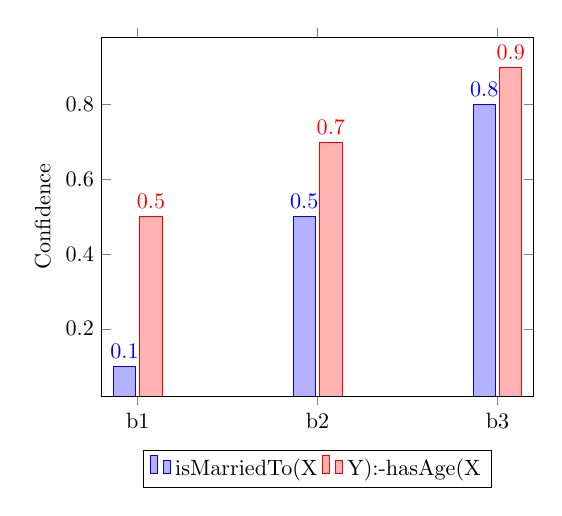
\begin{tikzpicture}[scale=0.8]
\begin{axis}[
    ybar,
    enlargelimits=0.10,
    legend style={at={(0.5,-0.15)},
      anchor=north,legend columns=-1},
    ylabel={Confidence},
    symbolic x coords={b1,b2,b3},
    xtick=data,
    nodes near coords,
    nodes near coords align={vertical},
    ]
\addplot coordinates {(b1,0.1) (b2,0.5) (b3,0.8)};
\addplot coordinates {(b1,0.5) (b2,0.7) (b3,0.9)};
\legend{isMarriedTo(X,Y):-hasAge(X,Z) , isMarriedTo(X,Y):-hasAge(X,Z)hasChild(X,A)}
\end{axis}
\end{tikzpicture}
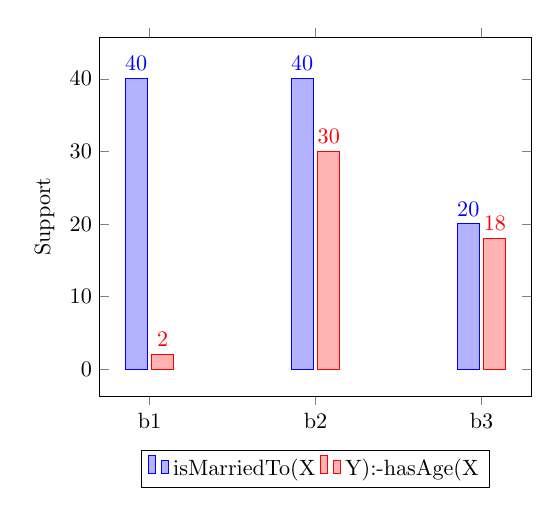
\begin{tikzpicture}[scale=0.8]
\begin{axis}[
    ybar,
    enlargelimits=0.15,
    legend style={at={(0.5,-0.15)},
      anchor=north,legend columns=-1},
    ylabel={Support},
    symbolic x coords={b1,b2,b3},
    xtick=data,
    nodes near coords,
    nodes near coords align={vertical},
    ]
\addplot coordinates {(b1,40) (b2,40) (b3,20)};
\addplot coordinates {(b1, 2) (b2,30) (b3,18)};
\legend{isMarriedTo(X,Y):-hasAge(X,Z), isMarriedTo(X,Y):-hasAge(X,Z)hasChild(X,A)}
\end{axis}
\end{tikzpicture}
\end{figure}

Adding a given predicate to the rule might not bring any gain or even loss in confidence to the base-rule, but when
bucketing per age, present a different confidence and support distribution and might even produce gain in confidence for
some specific buckets.

Nevertheless, adding a predicate with no correlation to the rule might not generate any gain. Thus, it's necessary to
carefully choose the relations and eventual constants and discard the ones with no correlation to the rule.  

\section{Contributions}
In this thesis, we propose a pre-processing step to build a graph we call correlation lattice for each numerical
property we want to for interesting intervals. In each graph, that has a numerical property as its root, we first
query the examples distribution on the numerical attribute, and build a histogram by discretizing them into $k$
buckets. Subsequently, we  pick a set of $c$ categorical properties that can be joined with the root, extract the
frequencies histogram and analyze how the distribution of sub-population created by joining them with the root is
affected. Afterwards, we try to combine the categories and check whether they still produce interesting sub-populations
creating a lattice, like in frequent set mining apriori algorithm.

We compare the distributions obtained from the frequencies histograms using information theoretical measures,
such as Kullback-Leibler divergence, as well as independence checks, such as Pearson's Chi-squared, in order to
measure the interestingness of adding literals to clauses.

Moreover, we discuss the pruning opportunities and also evaluate different heuristics and interestingness measures and
their efficiency in finding rules with numerical intervals. 

\begin{comment}
In a clause containing a numerical attribute in the body, we can obtain a support and confidence as well as support
value for each of the buckets. Therewith, we can search the most interesting intervals that satisfies the support and
confidence thresholds
\end{comment}

With information about different example distributions contained in the generated lattice, once we add one of the root
properties during the core ILP algorithm, we can then search for the most interesting categorical properties that could
result in different confidence distributions. For every categorical property, we can also suggest the most interesting
constants and other categorical properties to be combined in a subcategory of both.

In summary, we present in this thesis three main contributions:

\begin{itemize}
 \item A measure of the interestingness of searching for a specific interval for a rule's numerical attribute
variable.
 \item The correlation lattice and its pruning methods.
 \item Experiments on Linked Open Data datasets.
\end{itemize}


\section{Outline}

\begin{comment}
 The remainder of this thesis is structured as follows. In
Chapter~\ref{ch:technical_background}, we provide technical background on
MapReduce and BigTable. In Chapter~\ref{ch:related_work}, we present a
summary of previous work in the areas of duplicate and near-duplicate detection,
information retrieval on web archives, and MapReduce applications in graph
processing. Following that, we state our problem and describe solutions in
Chapter~\ref{ch:redundancy_control}. In Chapter~\ref{ch:mapreduce_impl}, we
describe an implementation of our solution using the MapReduce framework. In
Chapter~\ref{ch:experiments}, we present our experimental results. We conclude
this thesis and outline directions of future research in Chapter~\ref{ch:future_work}.
\end{comment}
 % Introduction

\chapter{Related Work}
\label{sec:rw-intro}

In this chapter relevant work related to the thesis topic will be briefly presented. In section 
~\ref{sec:rw-lp} we introduce important logic programming concepts, and in section~\ref{sec:rw-ilp} we discuss in
more details how Inductive Logic Programming (ILP) works. Later, in section~\ref{sec:rw-arm} we briefly present
association rule mining highlighting concepts relevant to this thesis. In section~\ref{sec:rw-discretization}, we
talk about discretization of numerical attributes and discuss the most popular unsupervised methods. After that, we
present in section~\ref{sec:rw-miningOptimizedRules} a method for mining rules optimized numerical intervals. In
section~\ref{sec:rw-infotheoreticmeasures}, we introduce the information-theoretical measures used in this thesis,
and finally, in sections~\ref{sec:rw-semanticWeb} and~\ref{sec:rw-lod}, we give a quick overview about Semantic Web
and Linked Open Data.


\section{Logic Programming}
\label{sec:rw-lp}

In this section, basic logic programming and deductive database terminology such as \emph{literal}, \emph{clause},
\emph{program clause}, \emph{datalog clause} and \emph{hypothesis} will be presented. We use terminology and
definitions described in \citet{DBLP:books/sp/Lloyd87} and \citet{LavracDz94}.

Firstly, it is important to
mention that variables are represented as uppercase letters followed by a string of lowercase letters and/or digits.
Function and predicate symbols (including constants) are lowercase letters also followed by a string of lowercase and/or
digits.

Following the An \emph{atomic formula} $L$ is a predicate symbol followed by a bracketed n-tuple of \emph{terms}. A
\emph{term} can
be
a variable or a function symbol followed by a bracketed n-tuple of terms. A constant is a function symbol of arity 0.
So
for example, if $f$, $g$, and $h$ are function symbols and $X$ a variable, then $g(X)$ is term, $f(g(X),h)$ is also a
term and $h$ is a \emph{constant}.

A \emph{literal} is an \emph{atomic formula} which can be negated or not. So both $L$ and its negation $\overline{L}$
are literals for any \emph{atomic formula} $L$. A clause $c$ is a disjunction of literals, for example:
\begin{center}
  $c=(L_1 \vee L_2 \vee \ldots \overline{L_{i}} \vee \overline{L_{i+1}} \vee \ldots) \equiv
 L_1 \vee L_2 \vee \ldots \leftarrow L_i \wedge L_{i+1} \wedge \ldots$
\end{center}

Such disjunction of literals can also be written in following way:
\begin{center}
 $\{L_1,L_2,\ldots,\overline{L_i},\overline{L_{i+1}},\ldots\}$ \\
$ L_1,L_2,\ldots \leftarrow L_i,L_{i+1},\ldots$
\end{center}

A \emph{program clause} is a clause which contains exactly one positive literal. That is, it has the form:
\begin{center}
 $\underbrace{T}_{head} \leftarrow \underbrace{L_1,L_2,\ldots}_{body}$
\end{center}

A \emph{Datalog clause} is a program clause with no function symbols with arity greater different from zero. That
means that only variables and constants can be used as predicate arguments. A datalog clause is considered \emph{safe}
if all the variables present in the head literal $T$ are also present in the body. Moreover, it may also allow negated
literals in the body, as long as every variable existent in a negated body literal are also be present in a
non-negated body literal.

Besides that, it is important to mention that Datalog rules support not only relational predicates but also
arithmetical, such as $=$, $\neq$, $>$, $<$, $\geq$, $\leq$, which improves the expressiveness of the language
allowing that, for instance, numerical attribute variables have their domain restricted to a specific interval.

\section{Inductive Logic Programming}
\label{sec:rw-ilp}

Inductive Logic Programming (ILP) is a machine learning technique that combines machine learning with the
logic programming representation. Given a known background knowledge and a set of training examples represented as a
logical database of facts (literals without any variables), an ILP system will learn a hypothesis in the form of a
logic program.

The clauses in the hypothesis aim at recognizing a concept $\mathcal{C}$, which is defined as a subset of objects
$\mathcal{C} \subseteq \mathcal{U}$. For example, $\mathcal{U}$ may be the set of all students in a University and
$\mathcal{C}$ all the students studying Informatics.
Concepts and objects are described in a description language $\mathcal{L}$, typically a subset of first-order logic,
but
various languages have also been used in ILP, including propositional logic and first order predicate calculus.

The training data for learning a concept $\mathcal{C}$ is a set of examples $\mathcal{E}$, where each examples is a
grounded fact
labeled as positive ($\oplus$) if the object is an instance of $\mathcal{C}$, or negative ($\ominus$) otherwise. We
denote the set
of positive examples as $\mathcal{E}^{+}$ and the set of negative examples as $\mathcal{E}^{-}$.

The background knowledge $\mathcal{B}$ is a prior knowledge which contributes in learning the hypothesis. It
indirectly
restricts the hypothesis search space, as  the learned hypothesis $\mathcal{H}$ should be consistent with the
background
knowledge as well as the training examples.

As defined in \citet{DBLP:journals/ml/LavracD96}, a hypothesis $\mathcal{H}$ is covers an example $e$ given a
background knowledge $\mathcal{B}$ ($covers(\mathcal{B} \cup \mathcal{H},e)$) if the example satisfies the hypothesis
and background knowledge. In logic programming where the $\mathcal{H}$ is a set of program clauses and an example is a
ground fact, it means that $e$ is entailed by $\mathcal{B} \cup \mathcal{H}$.

\begin{center}
 $covers(\mathcal{B} \cup \mathcal{H},e)=true \quad$ if $\quad \mathcal{B} \cup \mathcal{H} \models e$
\end{center}

We can also define a covering function for a set of examples which returns a a subset with the examples entailed by
$\mathcal{B} \cup \mathcal{H}$:

\begin{center}
 $covers(\mathcal{B} \cup \mathcal{H},\mathcal{E})=\{e \in \mathcal{E} | \mathcal{B} \cup \mathcal{H} \models e\}$
\end{center}

Therewith, we can define two important concepts in inductive learning:

\begin{itemize}
 \item Completeness: A hypothesis $\mathcal{H}$ is complete with respect to background knowledge $\mathcal{B}$ and
examples $\mathcal{E}$ if all the positive examples are covered, or in other words:
$covers(\mathcal{B},\mathcal{H},\mathcal{E}^{+})=\mathcal{E}^{+}$
 \item Consistency: A hypothesis $\mathcal{H}$ is consistent with respect to background knowledge $\mathcal{B}$ and
examples $\mathcal{E}$ if no negative examples are covered, or in other words:
$covers(\mathcal{B},\mathcal{H},\mathcal{E}^{-})=\emptyset$
\end{itemize}

The objective of learning a concept requires a hypothesis that is complete and consistent with respect to the given
concept training examples and background knowledge. The example shown in table~\ref{tab:ilpExample} illustrates a simple
problem of learning a hypothesis for the target relation
$daughter(X,Y)$.

\begin{table}[h!]
\caption{A simple ILP problem: learning the \emph{daughter} relation \citep{DBLP:journals/ml/LavracD96} .}
  \begin{center}
      \begin{tabular}{ r | l }
      \toprule
      \textbf{Training Examples} & \textbf{Background Knowledge}\\
      \midrule
      daughter(mary,ann) $\oplus$	& parent(ann,mary).	\\
      daughter(eve,tom) $\oplus$	& parent(ann,tom).	\\
      daughter(tom,ann) $\ominus$ 	& parent(tom,eve).	\\
      daughter(eve,ann) $\ominus$	& parent(tom,ian).	\\
					& female(ann).		\\
					& female(mary).		\\
					& female(eve).		\\
      \bottomrule
      \end{tabular}
  \label{tab:ilpExample}
  \end{center}
\end{table}

If we consider, for example, the language of safe datalog clauses, it is possible to formulate the following complete
and consistent hypothesis:

\begin{center}
  $\mathcal{H} = daughter(X,Y)$ :- $female(X),parent(Y,X)$ 
\end{center}

\subsection{Searching the Hypothesis Space}

In ILP, the hypothesis space is determined by the language of the programs $\mathcal{L}$ consisting of the possible
program clauses allowed by the language. Also, the vocabulary of predicate symbols is determined by the predicates
from the background knowledge $\mathcal{B}$.

\citet{DBLP:journals/ml/LavracD96} structures the search space with partial ordering of clauses based on
$\theta$-subsumption, in order to systematically search the program clauses space. A clause $c$ $\theta$-subsumes $c'$
if there's a substitution $\theta$ such that clause $c\theta \subseteq c'$. This also introduces a notion of generality,
where clause $c$ is at least as generally as $c'$, or in other words, $c'$ is a specialization of $c$.

For example, if we have the following $c$ and $c'$:
\begin{align*}
  c &= daughter(X,Y) \text{ :- } parent(Y,X) \\
  c'&= daughter(X,Y )\text{ :- } female(X),parent(Y,X)
\end{align*}

we know that for that $c'$ is a specialization of $c$ because for $\theta=\emptyset$, $c \subset c'$ since:
\begin{center}
$\{daughter(X,Y),\neg parent(Y,X)\} \subset \{daughter(X,Y),\neg female(X),\neg parent(Y,X)\}$ 
\end{center}

To better illustrate this, if we have:
\begin{align*}
  c &= livesIn(X,Y) \text{ :- } marriedTo(X,Z),livesIn(Z,Y)\\
  c'&=livesIn(X,germany) \text{ :- } marriedTo(X,Z),livesIn(Z,germany)
\end{align*}

we know that $c'$ is a specialization of $c$ because with the substitution $\theta=\{Y/germany\}$, $c\theta=c'$.

This notion gives us an important property that can be used for pruning parts of the search space:

\begin{itemize}
 \item When generalizing from $c$ to $c'$, all the examples covered by $c$ are also covered by $c'$. So if $c$ is
inconsistent, then all its generalizations are inconsistent as well.
  \item When specializing from $c$ to $c'$, an example not covered by $c$ will neither be covered by $c'$. So if $c'$
does not cover any positive examples, neither do any its specializations.
\end{itemize}

These properties are the basis for two main search approaches:

\begin{itemize}
 \item Bottom-up: starts with less general clauses and searches least general generalizations
 \item Top-down: starts with more general clauses and searches for most general consistent specializations
\end{itemize}

As in this thesis we work only with the top-down approach, we will discuss it in more details in the next subsection.
Further information about bottow-up approach can be found in \citet{DBLP:journals/ml/LavracD96}.

\subsection{Top-Down ILP}

The search space of program clauses can be viewed as a lattice, structured by $\theta$-subsumption generality
ordering. Such a lattice is called a \emph{refinement graph}, which can be used to direct the search from most general
to specific hypothesis. Figure~\ref{fig:refinementGraph} illustrates a part of the refinement graph for the
family relation example shown in table~\ref{tab:ilpExample}.

\begin{figure}[h!]
\begin{center}
  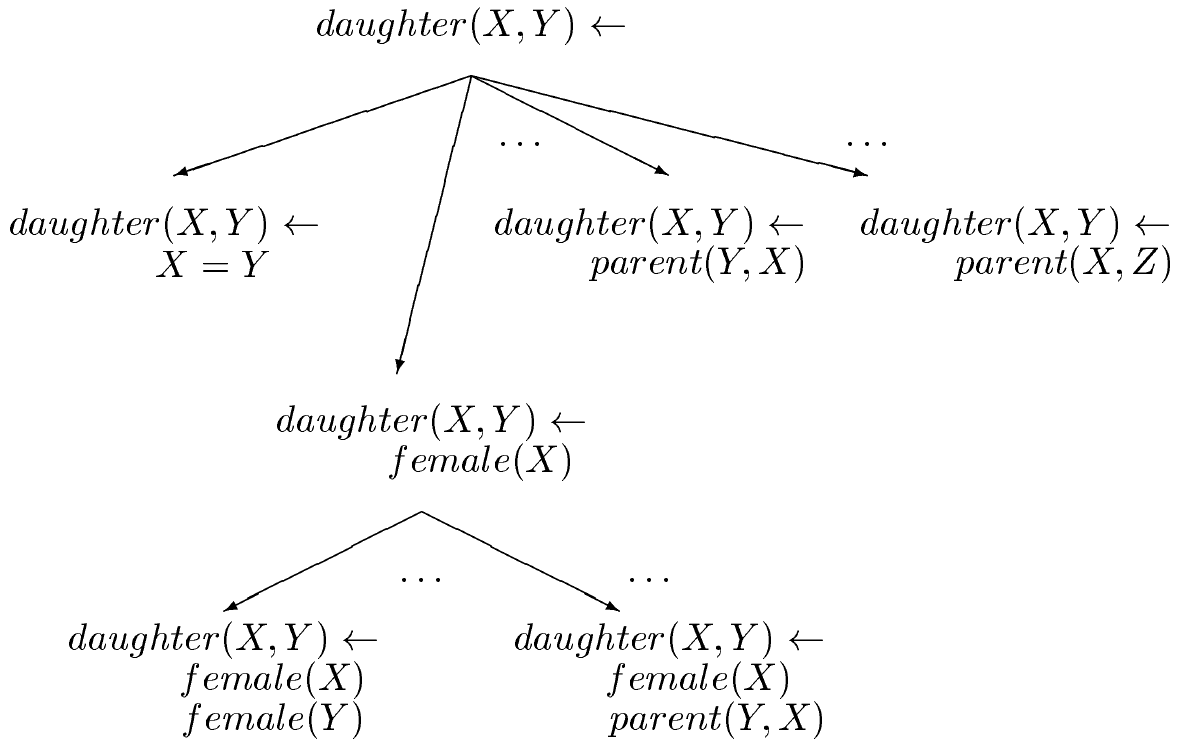
\includegraphics[width=0.7\linewidth]{./Figures/refinementGraph.png}
\end{center}
\caption{Part of the refinement graph for the family relations problem\citep{DBLP:journals/ml/LavracD96}.}
\label{fig:refinementGraph}
\end{figure}

In such a graph, nodes are program clauses and arcs are refinement operations, which can be of two kinds: apply
a substitution on the clause; add a literal to the body of the clause.

The top-down algorithm consists basically of a specialization loop that refines a clause ensuring consistency
embedded inside a covering loop that adds clauses to the hypothesis ensuring completeness. Each loop has a stopping
criterion, the covering loop iterates until it satisfies a sufficiency criterion and the specialization loop iterates
until it satisfies a necessity criterion. The algorithm~\ref{alg:topDownILP} shows in more details how the generic
top-down ILP works.

\begin{algorithm}[!h]
  \caption{Generic top-down specialization ILP algorithm \citep{DBLP:journals/ml/LavracD96}.}
  \SetKwFunction{executeQuery}
  \KwIn{\textbf{Input:} $\mathcal{E}$: Training examples, $\mathcal{B}$: Background knowledge \\ }
  \KwResult{$\mathcal{H}$: Learned hypothesis}

  \tcp{Initialize the current training set and hypothesis}
  $\mathcal{E}_{cur} \leftarrow \mathcal{E}$ \;
  $\mathcal{H} \leftarrow \emptyset$ \;
  \Repeat(Covering Loop){Sufficiency Stopping Criterion is satisfied} {
    \tcp{Initialize clause with empty body}
    $c \leftarrow T$ :- $\emptyset$ \;
    \Repeat(Specialization Loop){Necessity Stopping Criterion is satisfied} {
      $c_{best} \leftarrow$ Best refinement of $c$;
      $c \leftarrow c_{best}$ \;
    } ()
    \tcp{Add clause to the hypothesis}
    $\mathcal{H} \leftarrow \mathcal{H} \cup \{c\}$ \;
    \tcp{Remove positive examples covered by the new hypothesis}
    $\mathcal{E}_{cur} \leftarrow \mathcal{E}_{cur} - covers(\mathcal{B} \cup \mathcal{H},\mathcal{E}_{cur}^{+})$ \;
  } ()
 \label{alg:topDownILP}
\end{algorithm}

In domains with perfect data, the stopping criteria require that all positive examples are covered (completeness) and
no
negative examples are covered (consistency). However, in practice, many datasets have imperfect data. Such
imperfection is usually of the following kinds, as described in \citet{DBLP:conf/aii/LavracD92}:

\begin{itemize}
  \item Noise: random errors in the training examples and background knowledge.
  \item Insufficiently covered example space: too sparse training examples from which it is difficult to reliably
detect correlations.
  \item Inexactness: inappropriate or insufficient description language which does not contain an exact description of
the target concept.
  \item Missing facts in the training example.
\end{itemize}

In order to avoid the effects of imperfect data, ILP can use heuristics as stopping criteria which tolerate
some level of incompleteness and inconsistency. The simplest heuristic is the expected accuracy of a clause, which is
defined as the probability that an example
covered by the clause is labeled as positive:
\begin{equation}
A(c)=P(e \in \mathcal{E}^{+}|c)=\cfrac{n^{+}(c)}{n^{+}(c)+n^{-}(c)} 
\end{equation}
where $n^{+}(c)$ is the number of positive and $n^{-}(c)$ the number of negative examples covered by $c$. 

\subsection{ILP Complexity}

As shown in \citet{DBLP:journals/ngc/GottlobLS99}, the complexity of ILP resides at the second level of polynomial
hierarchy and it is $\Sigma_2^P$-complete. $\Sigma_2^P$ means that it has complexity $NP^{NP}$, and that happens
because there are two interlaced sources of $NP$ complexity class:
\begin{itemize}
 \item Choice problem, which is $NP$
 \item Checking problem, which is $co$-$NP$
\end{itemize}

The choice problem, in ILP, is the the problem of searching in the hypothesis space, while the checking problem is the
problem of testing a given hypothesis. Since ILP has a great complexity, it is appropriate to employ various techniques
with the objective of reducing runtime.

One popular strategy is the limitation of the number of literals allowed in a clause, which limits the number of
levels, which is easy to implement and can drastically reduce the size of the hypothesis search space, nevertheless, it
may also reduce the quality of the learned hypothesis. Another popular strategy is the data sampling. When well applied,
this can be a very good alternative, however, with semantic data, it can be very tricky to make a good sample without
significant loss of information. There are several different sampling techniques for semantic data, however, it is out
of the scope of this thesis.

%\section{First Order Inductive Learning}
%\cite{DBLP:journals/ml/Quinlan9}
%\cite{DBLP:conf/ecml/QuinlanC93}

\section{Association Rule Mining}
\label{sec:rw-arm}

Association Rule Mining, as described in~\citet{Agrawal:1993:MAR:170036.170072}, is method for discovering interesting
relations between variables in large databases. It is intended to work on a database composed by a set of transactions
$\mathcal{D}=\{t_1,t_2,\ldots,t_m\}$ and a set of items $\mathcal{I}=\{i_1,i_2,\ldots,i_n\}$. Each transaction
$\mathcal{T}$ consists of a set of items which is subset of $I$, which is usually represented by a binary vector of size
$n$ indicating the presence of absence of items in the
transaction.

The objective of association rule mining is to learn inference rules of the form $X \Rightarrow Y$, where $X,Y
\subseteq I$ and $X \cap Y = \emptyset$. Rules are selected according to various interestingness measures that will be
subsequently discussed.

\subsection{Measures}

In this subsection we will discuss measures used for selecting interesting rules in the mining process.

As defined in~\citet{Agrawal:1993:MAR:170036.170072}, a transaction $\mathcal{T}$ supports an itemset
$\mathcal{X} \subseteq \mathcal{I}$ if $\mathcal{X} \subseteq
\mathcal{T}$. The support measure $supp(X)$ is the defined as the ratio between the number of transactions supporting
$X$ and the total size of the database $\mathcal{D}$:

\begin{equation}
 supp(X)=\cfrac{|\{ \mathcal{T} \in \mathcal{D} | X \subseteq \mathcal{T} \}|}{|\mathcal{D}|}
\end{equation}

The support of a rule $X \Rightarrow Y$ is defined as:

\begin{equation}
 supp(X \Rightarrow Y)=supp(X \cup Y)
\end{equation}

The confidence of a rule $X \Rightarrow Y$, which can may be interpreted as the probability of the the head given the
body $P(Y|X)$, is defined as:

\begin{equation}
 conf(X \Rightarrow Y)=\cfrac{supp(X \cup Y)}{sup(X)}
\end{equation}

%Need to cite who invented lift
Confidence and support are the two measures used in classical association rule mining. Albeit, there are other
relevant
measures such as \emph{lift}. It measures how different the observed rule support is in comparison to that expected if
$X$ and $Y$ were independent:

\begin{equation}
 lift(X \Rightarrow Y)=\cfrac{supp(X \Rightarrow Y)}{supp(X)supp(Y)}
\end{equation}

A lift value 1 would imply that $X$ and $Y$ are independent, therefore any rule involving both itemsets does not make
sense. A lift value greater than 1, provides information about the level of dependence between both variables. Higher
lift values makes a rule potentially more interesting.

\subsection{Anti-monotonicity of Support}

An important characteristic of the support measure is the anti-monotonicity. It means that for any itemset $X
\subseteq \mathcal{I}$ if we have another itemset $Y \subseteq \mathcal{I}$ such that $X \subseteq Y$, then the
support
of $Y$ cannot be greater than the support of $X$. In other words, all subsets from a frequent itemset are also
frequent,
and all supersets from an infrequent item are also infrequent.

When searching for frequent itemsets, this characteristic plays a key role in pruning the search space, which grows
exponentially with the number of items $n$. The set of possible itemsets is the power set over $\mathcal{I}$, which
has
size $2^n-1$. As association rules are usually required to satisfy a specified minimum support, if we know that a
given
itemset does not satisfy it, we can automatically prune all its supersets.

\subsection{Itemset Lattice}

The problem of searching frequent itemsets (FI), i.e., itemsets that satisfy the specified minimum support, can be
structured in a lattice. Firstly, an itemset is frequent if it has support greater or equal than an arbitrarily
specified minimum support.

There are two special kinds of itemsets:
\begin{itemize}
 \item Maximal frequent itemset (MFI): a frequent itemset is maximal if none of its immediate supersets are frequent.
 \item Closed frequent itemset (CFI): a frequent itemset is closed if all of its immediate supersets have lower
support.
\end{itemize}

Each of these kinds of itemsets has an special property. By knowing all the maximal itemsets of a database, we
also know all the frequent itemsets. Nevertheless, it is not possible to know the support of each of the frequent
itemsets. By knowing all the closed itemsets of a database, it is possible to know the all the frequent itemsets as
well as their supports.

In the example of database $\mathcal{D}$ shown in Table~\ref{tab:itemsetLattice} with the resulting itemset lattice
shown in Figure~\ref{fig:itemsetLattice}, frequent itemsets are shown with thicker border. The minimum support
threshold is set to $2/5$, so the frequent itemsets are the ones with frequency greater than or equal to 2. For this
example, we would have as maximal itemset $\{ABCE\}$ and as closed itemsets $\{ABCE, BCE, BE\}$

\begin{table}[h!]
  \begin{center}
      \begin{tabular}{ c | l l l l }
      \toprule
      \textbf{TID} & \multicolumn{4}{c}{\textbf{Items}} \\
      \midrule
	1	& A & C & D & \\
	2 	& B & C & E & \\
	3	& A & B & C & E \\
	4 	& B & E &   & \\
	5	& A & B & C & E \\
      \bottomrule
      \end{tabular}
  \caption{Example of transaction database $\mathcal{D}$ \citep{Pasquier99efficientmining}}
  \label{tab:itemsetLattice}
 \end{center}
\end{table}

\begin{figure}[!h]
  \caption{Itemset Lattice example~\citep{Pasquier99efficientmining}.}
  \centering
  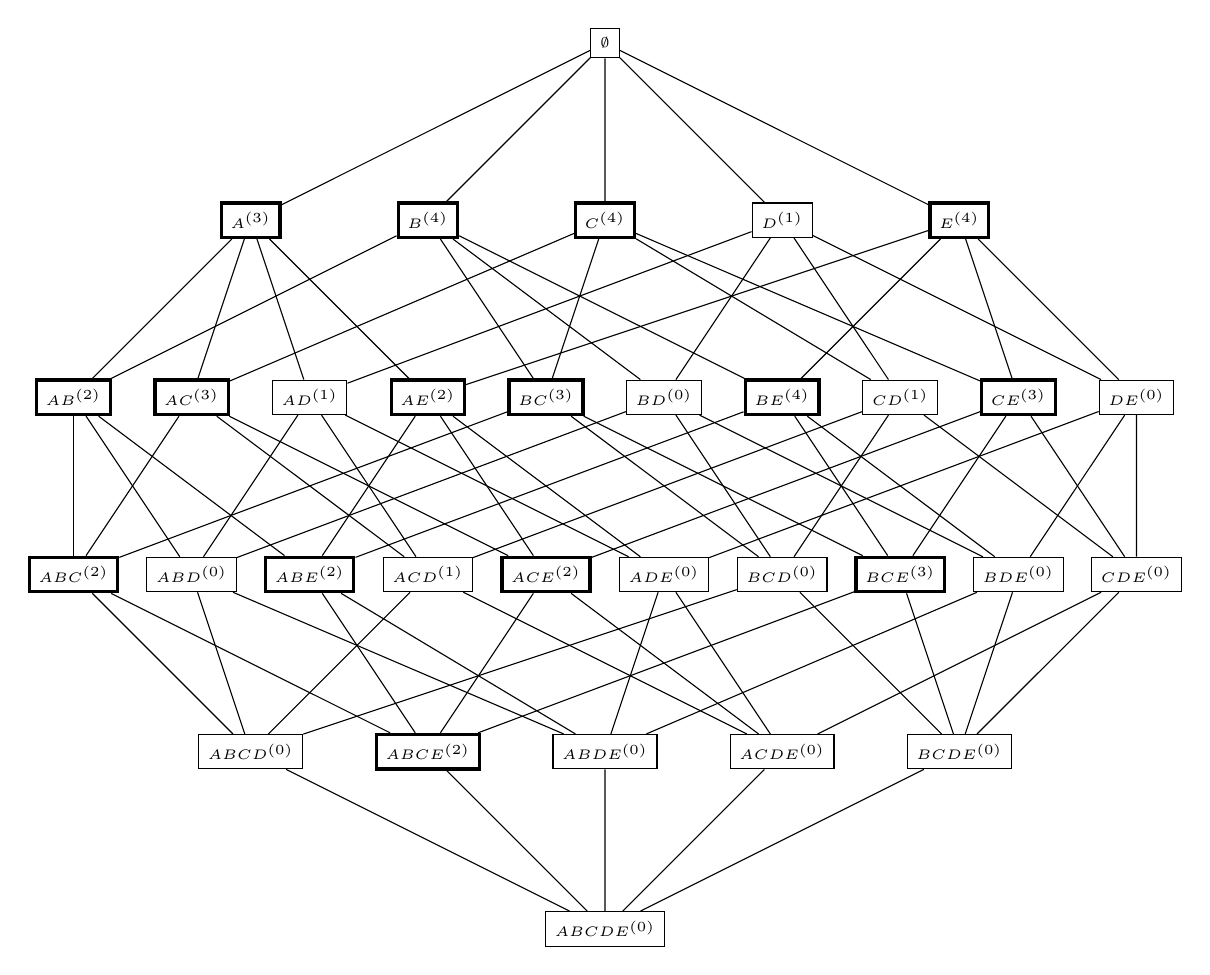
\begin{tikzpicture}[scale=0.75,auto=center,every node/.style={draw=black, font=\tiny}]
    \node (n0) at (11,15) {$\emptyset$};

    \node (A)[very thick] 	at (5,12)  {$A^{(3)}$};
    \node (B)[very thick] 	at (8,12)  {$B^{(4)}$};
    \node (C)[very thick]	at (11,12) {$C^{(4)}$};
    \node (D)			at (14,12) {$D^{(1)}$};
    \node (E)[very thick]	at (17,12) {$E^{(4)}$};

    \node (AB)[very thick] 	at (2,9)  {$AB^{(2)}$};
    \node (AC)[very thick] 	at (4,9)  {$AC^{(3)}$};
    \node (AD) 			at (6,9)  {$AD^{(1)}$};
    \node (AE)[very thick] 	at (8,9)  {$AE^{(2)}$};
    \node (BC)[very thick] 	at (10,9) {$BC^{(3)}$};
    \node (BD) 			at (12,9) {$BD^{(0)}$};
    \node (BE)[very thick] 	at (14,9) {$BE^{(4)}$};
    \node (CD) 			at (16,9) {$CD^{(1)}$};
    \node (CE)[very thick] 	at (18,9) {$CE^{(3)}$};
    \node (DE) 			at (20,9) {$DE^{(0)}$};

    \node (ABC)[very thick] 	at (2,6)  {$ABC^{(2)}$};
    \node (ABD) 		at (4,6)  {$ABD^{(0)}$};
    \node (ABE)[very thick] 	at (6,6)  {$ABE^{(2)}$};
    \node (ACD) 		at (8,6)  {$ACD^{(1)}$};
    \node (ACE)[very thick] 	at (10,6) {$ACE^{(2)}$};
    \node (ADE) 		at (12,6) {$ADE^{(0)}$};
    \node (BCD) 		at (14,6) {$BCD^{(0)}$};
    \node (BCE)[very thick] 	at (16,6) {$BCE^{(3)}$};
    \node (BDE) 		at (18,6) {$BDE^{(0)}$};
    \node (CDE) 		at (20,6) {$CDE^{(0)}$};

    \node (ABCD) 		at (5,3)  {$ABCD^{(0)}$};
    \node (ABCE)[very thick] 	at (8,3)  {$ABCE^{(2)}$};
    \node (ABDE) 		at (11,3) {$ABDE^{(0)}$};
    \node (ACDE) 		at (14,3) {$ACDE^{(0)}$};
    \node (BCDE) 		at (17,3) {$BCDE^{(0)}$};

    \node (ABCDE) at (11,0) {$ABCDE^{(0)}$};

    \foreach \from/\to in
      {n0/A,n0/B,n0/C,n0/D,n0/E,
       A/AB, A/AC, A/AD, A/AE, 
       B/AB, B/BC, B/BD, B/BE, 
       C/AC, C/BC, C/CD, C/CE,
       D/AD, D/BD, D/CD, D/DE,
       E/AE, E/BE, E/CE, E/DE,
       AB/ABC, AB/ABD, AB/ABE,
       AC/ABC, AC/ACD, AC/ACE,
       AD/ABD, AD/ACD, AD/ADE,
       AE/ABE, AE/ACE, AE/ADE,
       BC/ABC, BC/BCD, BC/BCE,
       BD/ABD, BD/BCD, BD/BDE,
       BE/ABE, BE/BCE, BE/BDE,
       CD/ACD, CD/BCD, CD/CDE,
       CE/ACE, CE/BCE, CE/CDE,
       DE/ADE, DE/BDE, DE/CDE,
       ABCD/ABC, ABCD/ABD, ABCD/ACD, ABCD/BCD,
       ABCE/ABC, ABCE/ABE, ABCE/ACE, ABCE/BCE,
       ABDE/ABD, ABDE/ABE, ABDE/ADE, ABDE/BDE,
       ACDE/ACD, ACDE/ACE, ACDE/ADE, ACDE/CDE,
       BCDE/BCD, BCDE/BCE, BCDE/BDE, BCDE/CDE,
       ABCDE/ABCD, ABCDE/ABCE, ABCDE/ABDE, ABCDE/ACDE, ABCDE/BCDE}  
    \draw (\from) -- (\to);
  \end{tikzpicture}
  \label{fig:itemsetLattice}
\end{figure}

\subsection{Apriori Algorithm}
The apriori algorithm, discussed in ~\citet{Pasquier99efficientmining}, is a method for searching frequent itemsets
which explores the anti-monotonic property of the support measure. It computes the itemsets support iteratively, by
ascending order of size. The process takes $k$ iterations where $k$ is the size of the largest frequent itemset. In each
iteration $i \leq k$, the database is scanned once and all the support of all itemsets of size $i$ are computed.

In the first iteration, all itemsets of size 1 have their supports computed. On the $1 < i \leq k$ subsequent
iterations, a set of candidates $C_i$ is created by joining the frequent itemsets of size $i-1$ found in the previous
iteration. Two itemsets of size $i$ can only join if they share $i-1$ items, so their union can form an itemset of
size
$i+1$. Only after finding the set of candidate itemsets $C_1$, the database is scanned in order to determine the
support of each of them. Algorithm~\ref{alg:apriori} shows in more details how the apriori algorithm works.

\begin{algorithm}[h!]
  \caption{Apriori frequent itemset discovery~\citep{Pasquier99efficientmining}.}
  \SetKwFunction{aprioriGen}
  \KwIn{\textbf{Input:} $\mathcal{D}$: Database of transactions \\}
  \KwResult{$\mathcal{H}$: Learned hypothesis}

  $L_1 \leftarrow$ Frequent itemsets of size 1 \;
  $L \leftarrow L_1$ \;
  $k \leftarrow 1$ \;
  \While{$L_{k-1} \neq \emptyset$}{
      $C_k \leftarrow$ \FuncSty{aprioriGen(}$L_{k-1}$\FuncSty{)} \;
      \ForAll{$t \in \mathcal{D}$}{
	$C_t \leftarrow \{ c | c \in C_k \wedge c \subseteq t\}$ \;
	\ForAll{$c \in C_t$}{
	  $c.frequency \leftarrow c.frequency + 1$ \;
	}
      }
      $L_k \leftarrow \{ c | c \in C_k \wedge c.frequency \geq minSupport\}$ \;
      $L \leftarrow L \cup L_k$ \;
      $k \leftarrow k+1$ \;
  }
  \Return{$L$} \;
 \label{alg:apriori}
\end{algorithm}

For the previous example of database from Table~\ref{tab:itemsetLattice}, the itemset lattice generated by the apriori
algorithm is shown in Figure~\ref{fig:aprioriLattice}. 

\begin{figure}[h!]
  \caption{Itemset Lattice generated by apriori algorithm for the example from Table~\ref{tab:itemsetLattice}}
  
  \centering
  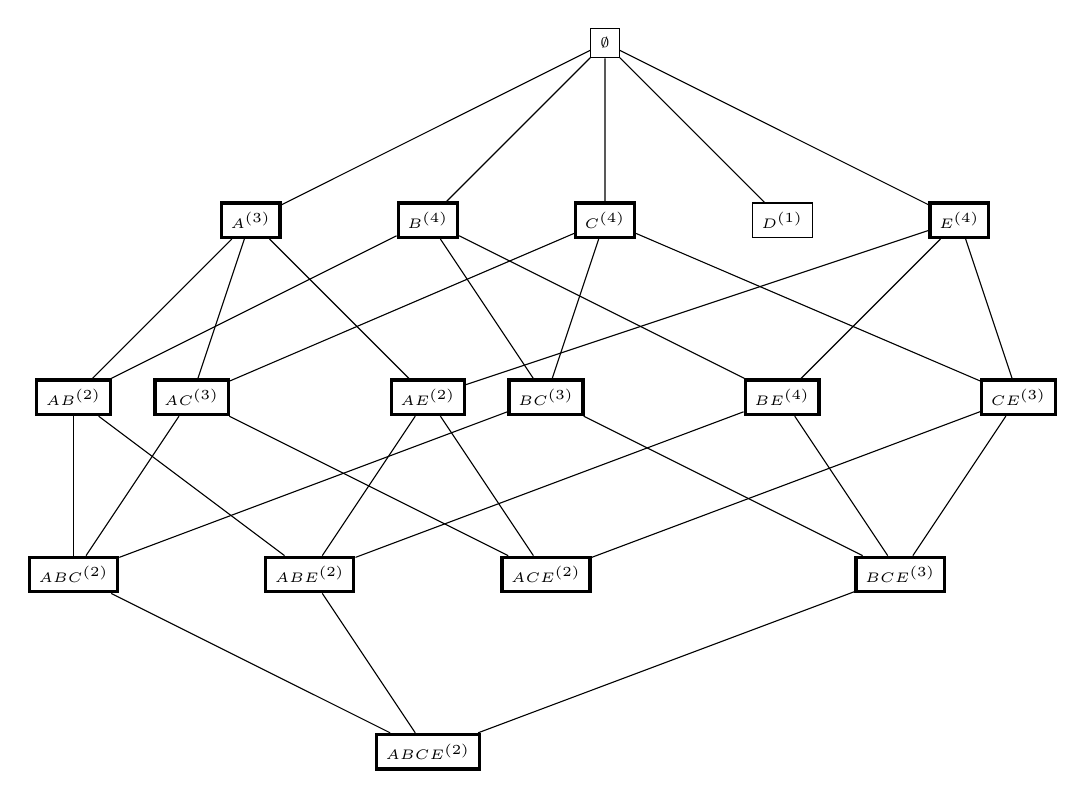
\begin{tikzpicture}[scale=0.75,auto=center,every node/.style={draw=black, font=\tiny}]
    \node (n0) at (11,15) {$\emptyset$};

    \node (A)[very thick] 	at (5,12)  {$A^{(3)}$};
    \node (B)[very thick] 	at (8,12)  {$B^{(4)}$};
    \node (C)[very thick]	at (11,12) {$C^{(4)}$};
    \node (D)			at (14,12) {$D^{(1)}$};
    \node (E)[very thick]	at (17,12) {$E^{(4)}$};

    \node (AB)[very thick] 	at (2,9)  {$AB^{(2)}$};
    \node (AC)[very thick] 	at (4,9)  {$AC^{(3)}$};
    \node (AE)[very thick] 	at (8,9)  {$AE^{(2)}$};
    \node (BC)[very thick] 	at (10,9) {$BC^{(3)}$};
    \node (BE)[very thick] 	at (14,9) {$BE^{(4)}$};
    \node (CE)[very thick] 	at (18,9) {$CE^{(3)}$};

    \node (ABC)[very thick] 	at (2,6)  {$ABC^{(2)}$};
    \node (ABE)[very thick] 	at (6,6)  {$ABE^{(2)}$};
    \node (ACE)[very thick] 	at (10,6) {$ACE^{(2)}$};
    \node (BCE)[very thick] 	at (16,6) {$BCE^{(3)}$};

    \node (ABCE)[very thick] 	at (8,3)  {$ABCE^{(2)}$};

    \foreach \from/\to in
      {n0/A,n0/B,n0/C,n0/D,n0/E,
       A/AB, A/AC, A/AE, 
       B/AB, B/BC, B/BE, 
       C/AC, C/BC, C/CE,
       E/AE, E/BE, E/CE,
       AB/ABC, AB/ABE,
       AC/ABC, AC/ACE,
       AE/ABE, AE/ACE,
       BC/ABC, BC/BCE,
       BE/ABE, BE/BCE,
       CE/ACE, CE/BCE,
       ABCE/ABC, ABCE/ABE, ABCE/BCE}  
    \draw (\from) -- (\to);
  \end{tikzpicture}
  \label{fig:aprioriLattice}
\end{figure}

As we will show later in Section~\ref{sec:correlation-lattice}, the itemset lattice and the apriori algorithm inspired
and served as base for the correlation lattice. Therefore, both structures look alike, and have similar building
processes.

\section{Discretization of Numerical Attributes}
\label{sec:rw-discretization}

Discretization of constinuous features is a very important tool which is frequently used in statistics, data mining
and machine learning. It is a pre-processing technique which is used for reducing the effects of observation errors.
It is basically a form of quantization where the original data values in a given interval are replaced by a
representative value of that interval.

Discretization techniques can be divided in supervised and unsupervised methods. The first requires the objects to
be labeled with classes, and the domain is discretized with the objetive of reducing the class entropies. The second
one does not consider object classes, only object frequencies. Unsupervised methods normally require the number of
buckets to be beforehand defined.

Various different supervised and unsupervised methods for the discretization of continuous features are discussed in
\citet{Dougherty95supervisedand}. To build the lattice, we don not use labels for the examples so we just use
unsupervised methods.

Supervised methods can be used for finding interesting intervals in the rules, by considering positive and negative
examples as labels. However, it is out of the scope of this thesis, thus we will not discuss these in detail.

\subsection{Equal Width}
This unsupervised discretization method consists of simply querying both the maximum and minimum values of the root's
numerical attribute, then splitting this interval into $k$ buckets of same width $w$:

\begin{equation}
 w=\cfrac{max-min}{k}
\end{equation}

It's the simples and most straightforward discretization method, but its main problem is that it is highly
sensitive to outliers that may drastically skew the resulting distribution.

\subsection{Equal Frequencies}
In this also unsupervised discretization method, the domain is divided in buckets with equal frequency. That is, given
a
total frequency $m$, the domain is discretized in $k$ buckets such that each has frequency $m/k$. Multiple
objects with same numerical attribute value might make it impossible to find bucket boundaries that equally
distribute the frequencies.

The greatest advantage of this method is that it always results in a distribution with highest possible entropy, i.e.,
distribution is always uniform or as close to uniformity as possible.

\section{Mining Optimized Rules for Numeric Attributes}
\label{sec:rw-miningOptimizedRules}

In \citet{Brin99miningoptimized}, a technique for efficiently learning association rules with interesting ranges for
numerical attributes is presented. It focuses on finding numerical intervals which optimize a specific interestingness
measure, given the confidence and support distribution of a rule along a numerical attribute. 

Such rules have the form $(A_1 \in [l_1,u_1]) \wedge C_1 \rightarrow C_2$, where
$A_1$ is a numerical attribute, $l_1$ and $u_1$ are the lower and upper boundaries of $A_1$, and $C_1$ and $C_2$
contain
only instantiated conditions.

The authors propose algorithms for determining values for the boundaries $l_1$ and $u_1$ for the following cases:

\begin{itemize}
 \item Optimized confidence: the rule confidence is maximized and  support of the condition $(A_1 \in [l_1,u_1])
\wedge
C_1$ is at least the specified minimum support.
  \item Optimized support: the support of the condition $(A_1 \in [l_1,u_1]) \wedge C_1$ is maximized and the rule
confidence is at least the specified minimum confidence.
  \item Optimized gain: the rule gain is maximized and the confidence is at least the specified minimum confidence.
\citet{Brin99miningoptimized} defines gain of a rule $r$ as $gain(r)= supp(r)*(conf(r)-minConf)$, where $minConf$ is the
confidence threshold.
\end{itemize}

In~\citet{Brin99miningoptimized}, the two dimensional case with two different numerical attributes is also discussed,
however, in this section we will focus on the single numerical attribute case.

Basically, it first takes the transactions with numerical attribute $A_1$ and discretizes its numerical domain of size
$n$ into $b < n$ buckets, in order to reduce the complexity of the algorithm. It uses a supervised bucketing algorithm,
which uses as labels ``$+$'' if the confidence value is greater than the threshold (positive gain), and ``$-$'', if it
is less (negative gain). This method does not compromise the optimality of the algorithm, as it collapses values with
similar labels together, generating $b$ buckets, each with its own support and confidence values.
Figure~\ref{fig:brinbucket} shows an example where a domain of size $n=6$ is discretized into $b=3$ buckets.

\begin{figure}
\begin{center}
  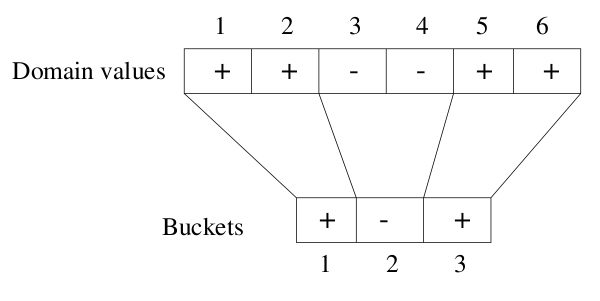
\includegraphics[width=0.5\linewidth]{./Figures/brin-bucket.png}
\end{center}
\caption{Example of buckets generated~\citep{Brin99miningoptimized}}
\label{fig:brinbucket}
\end{figure}

Algorithm~\ref{alg:brin} shows how the proposed one-dimensional algorithm works for gain optimization.
Figure~\ref{fig:optgain} illustrates that with an example with $b=6$ buckets, with confidence values $10$, $-15$, $20$,
$-15$, $20$, and $-15$. $PSet$ is the optimized gain set containing $i-1$ intervals, and $NSet$ contains the
remaining intervals not stored in $PSet$. These sets are represented before and after the iterations $i=1$ and $i=2$.
As shown in the figure, any optimized interval contained in $PSet$ has positive gain, and its neighboring intervals
have negative gain.

\begin{algorithm}[h!]
 \caption{Algorithm for computing optimized gain set~\citep{Brin99miningoptimized}}
 \label{alg:brin}
 \KwIn{\textbf{Input:} $b$: number of buckets, $k$: maximum number of optimum intervals}
  $PSet \leftarrow \emptyset$\;
  $NSet \leftarrow \{[1,b]\}$\;
  \For{$i \leftarrow 1$ to $k$} {
      Let $P_q$ be the interval in $PSet$ with the smallest value for $gain(min(P_q))$\;
      Let $N_q$ be the interval in $NSet$ with the smallest value for $gain(max(N_q))$\;
      \eIf{$gain(min(P_q))+gain(max(N_q)) < 0$}{
	  Delete $P_q$ from $PSet$\;
	  Split $P_q$ into three sub-intervals (with $min(P_q)$ as the middle interval)\;
	  Insert the first and third intervals to $PSet$ and second interval to $NSet$\;
      }{
	  Delete $N_q$ from $NSet$;
	  Split $N_q$ into three sub-intervals (with $max(N_q)$ as the middle interval)\;
	  Insert the first and third intervals to $NSet$ and second interval to $PSet$\;
      }
  }
  \Return $PSet$\;
\end{algorithm}

\begin{figure}
\begin{center}
  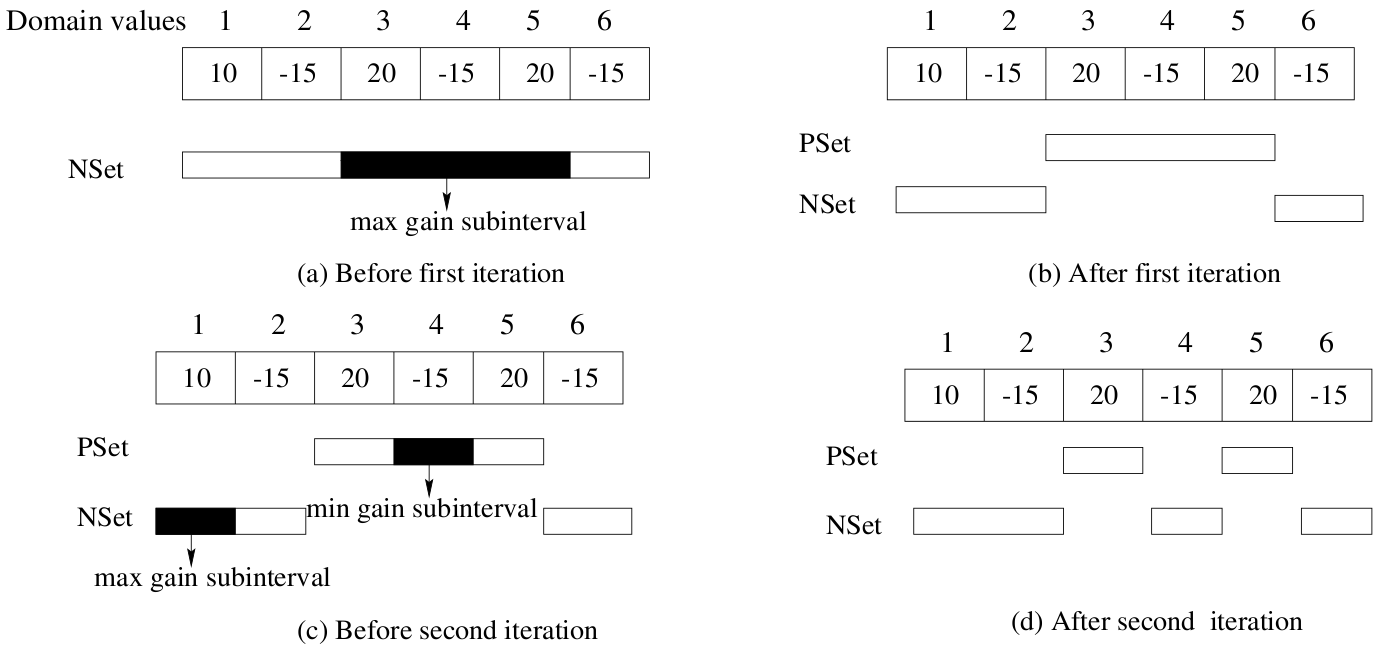
\includegraphics[width=1\linewidth]{./Figures/optgain1d.png}
\end{center}
\caption{Execution trace of procedure shown in Algorithm~\ref{alg:brin}. (a) Before first iteration, (b) after first
iteration, (c) before second iteration, and (d) after second iteration\citep{Brin99miningoptimized}.}
\label{fig:optgain}
\end{figure}

It is important to highlight that this technique does not have the same purpose of the work presented in this thesis.
While \citet{Brin99miningoptimized} focuses on finding the optimal interval with respect to a given measure, assuming
that we already have support and confidence distribution along the numerical attribute, in this thesis, we focus on
identifying rules which potentially have sub-interval with confidence gain in relation to its base rule, before we
actually query the support and confidence distributions, which is very expensive, pruning rules that have no
correlation to the numerical attribute to be investigated. 

\section{Information-Theoretic Measures}
\label{sec:rw-infotheoreticmeasures}

Information-theoretic measures are widely used in various different learning processes. Its importance lies on its
power
to measure importance of attributes and relationships between attributes. An attribute is considered important in data
mining if regularities are encountered in smaller populations obtained based on the values of such attribute, but not
in
the larger population. Such regularities are identifiable by lower entropy values, indicating that interesting
attributes lead to entropy reduction. More specifically, the entropy reduction is the difference between the entropy
of
the decision attribute and the conditional entropy of the decision attribute given a particular attribute, whose
importance we want to investigate.

Let's say we have $X$ as decision attribute and it divides the set of objects $\mathcal{U}$ into a group of disjoint
subsets defined by the value $x \in \mathcal{X}$ of $X$, where $\mathcal{X}$ is the non-empty set of values for
$X$. Also, let's define $I_X : \mathcal{U} \rightarrow \mathcal{X}$ is an information function that gives the value of
attribute $X$ for an object $t \in \mathcal{U}$. The set of objects $m(X=x) \subseteq \mathcal{U}$, whose value for
$X$
is $x$ is defined as follows:

\begin{equation}
 m(X=x)=m(x)=\{t \in \mathcal{U} | I_X(t)=x\}
\end{equation}

With that, the probability distribution of $X$ is defined by:

\begin{equation}
 P(X=x)=P(x)=\cfrac{|m(x)|}{|\mathcal{U}|},\quad x \in \mathcal{X}
\end{equation}

Information theoretic measures are defined over probability distributions. They can measure the importance of an
attribute, attribute association, dissimilarity, or similarity of populations. In the next subsections, we will
discuss some of the most important measures.

\subsection{Shannon's Entropy}

The Shannon's entropy measure $H$ is a non-negative function which may be interpreted as a measure of the information
content or uncertainty about an attribute $X$. It is defined over a probability distribution of $X$:

\begin{equation}
\begin{split}
 H(P(X))=H(X)&=E_{P(X)}[-logP(X)] \\
 &=-\sum_{x \in \mathcal{X}}P(x)logP(x)
\end{split} 
\end{equation}

The entropy of $X$ is maximum if its probability distribution is uniform, and minimum if the whole population is
concentrated on a specific value $x_c \in \mathcal{X}$, i.e., $P(x_c)=1$ and $P(x)=0, x \neq x_c$. The higher the
entropy,the higher the uncertainty about $X$'s attribute value, and an entropy of zero means complete certainty about
the value of $X$ since $P(x_c)=1$.

\subsection{Kullback-Leibler Divergence}
\label{sec:kldiv}

The Kullback-Leibler divergence~\citep{Kullback51klDivergence} $D(P||Q)$ between the population
distributions $P(X)$ and $Q(X)$ measures the degree
of deviation of $P$ from another distribution $Q$:

\begin{equation}
\begin{split}
 D_{KL}(P||Q)&=E_{P(X)}\left[\cfrac{P(X)}{Q(X)}\right] \\
 &=\sum_{x \in \mathcal{X}}P(x)log\left(\cfrac{P(x)}{Q(x)}\right)
\end{split} 
\end{equation}

This divergence measure is a premetric but not a metric distance. It is non-negative and it becomes zero if
$P(x)=Q(x)$,
$\forall x \in \mathcal{X}$, but it does not satisfy the symmetry and the triangle inequality properties.

There are symmetrized divergence measures based on the Kullback-Leibler, e.g. the $J$-divergence~\ref{eq:jDiv} and the
Jensen-Shannon divergence~\ref{eq:jensenShannon}:

\begin{equation} \label{eq:jDiv}
  D_{J}(P||Q) = D_{KL}(P||Q) + D_{KL}(Q||P)
\end{equation}
\begin{equation} \label{eq:jensenShannon}
  D_{JS}(P||Q) = \cfrac{1}{2}D_{KL}(P||M) + \cfrac{1}{2}D_{KL}(Q||M)
\end{equation}

where M is the average of the two distributions, $M=\cfrac{1}{2}(P+Q)$.

The Jensen-Shannon divergence also has the advantage that the difference is always a finite value ($0 \leq
D_{JS}(P||Q) \leq 1$, for the base-2 logarithm). Although, it still does not satisfy the triangle inequality property,
its square root does and, therefore, is a metric. Further details about these divergence measures are presented
in~\citet{17795}, \citet{Vinh:2010:ITM:1953011.1953024}, and~\citet{guiasu1977information}.

\subsection{Mutual Information}

The divergence measure can be used for computing the degree of independence between two attributes $X$ and $Y$. This
is
done by simply measuring the divergence between the observed joined distribution $P(X,Y)$ and the independent
distribution formed by the marginals $P(X)P(Y)$. We call such measure mutual information:

\begin{equation} \label{eq:mutualInformation}
\begin{split}
 MI(X;Y)&=D(P(X,Y)||P(X)P(Y)) \\
 &=E_{P(X,Y)}\left[ log\cfrac{P(x,y)}{P(x)P(y)} \right] \\
 &=\sum_{x \in \mathcal{X}} \sum_{y \in \mathcal{Y}} P(x,y)log\cfrac{P(x,y)}{P(x)P(y)}
\end{split}
\end{equation}

Completely independent attributes have mutual information zero, and the greater the level of dependence, the greater
the mutual information.

\section{Semantic Web Applications}
\label{sec:rw-semanticWeb}

The Semantic Web is, according to its official website\footnote{\url{http://www.w3.org/standards/semanticweb/}}, a
technology created by the World Wide Web Consortium (W3C) to enable the so-called ``Web of data'', enabling computers
to do more useful work and develop systems that can support trusted interactions over the network. 

It consists of a set of technologies and formats which aim to make web resources more readily accessible to automated
processes. The Semantic Web Stack, in Figure~\ref{fig:sematicWebLayer}\footnote{Semantic Web - XML2000, slide 10".
W3C: \url{http://www.w3.org/2000/Talks/1206-xml2k-tbl/slide10-0.html}}, illustrates the semantic web architecture
showing how its standards are organized and how it extends the classical hypertext web.

\begin{figure}
\begin{center}
  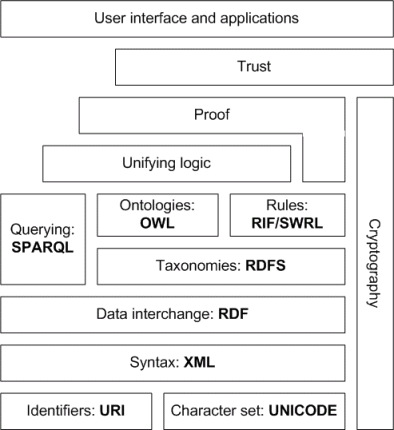
\includegraphics[width=0.5\linewidth]{./Figures/Semantic-web-stack.png}
\end{center}
\caption{Semantic Web stack}
\label{fig:sematicWebLayer}
\end{figure}

\begin{itemize}
 \item Resource Description Framework (RDF): a framework for creating statements in the form of triples composed by
subject, predicate and object. It uses URIs to name the predicates as well as the entities, which may be the subject
or
object in a triple. RDF can be encoded in a variety of formats, such as RDF/XML, N3, Turtle and N-Triples.
 \item RDF Schema (RDFS): a RDF vocabulary description language which provides basic elements for the description of
ontologies (or RDF vocabularies) intended to structure RDF resources known as constructs (RDFS classes, associated
properties, and utility properties).
 \item Web Ontology Language (OWL): a semantic markup language for publishing and sharing ontologies on the web. It is
a
vocabulary extension of RDF that allows an ontology to be described with a set of axioms which places constraints on
classes and the types of relationships permitted between them.
 \item SPARQL: an RDF query language for databases which can be used to express queries across diverse data sources.
It
consists of triple patterns, conjunctions, disjunctions and optional patterns. 
 \item Rule Interchange Format (RIF): defines a standard for exchanging rules among rule systems. It focuses on
exchange rather than defining a single one-fits-all rule language, different databases might have different
characteristics with different necessities.
  \item Semantic Web Rule Language (SWRL): a proposal for rule language combining sublanguages of OWL with the
Unary/Binary Datolog Rule Markup Language\footnote{\url{http://ruleml.org/}} (RuleML), which specifies different
derivation rules via XML Schema.
\end{itemize}

%ruleml.org/talks/RuleML-Family-PPSWR06-talk-up.ppt

%http://ruleml.org/1.0/exa/

\section{Linked Open Data Applications}
\label{sec:rw-lod}

The Semantic Web does not need only access to reachable and manageable data in a standard format, but also
relationships among data from different sources. Therewith, it is possible to create a huge collection of interrelated
datasets in the Web, also referred as Linked Data.

\begin{figure}[h!]
\begin{center}
  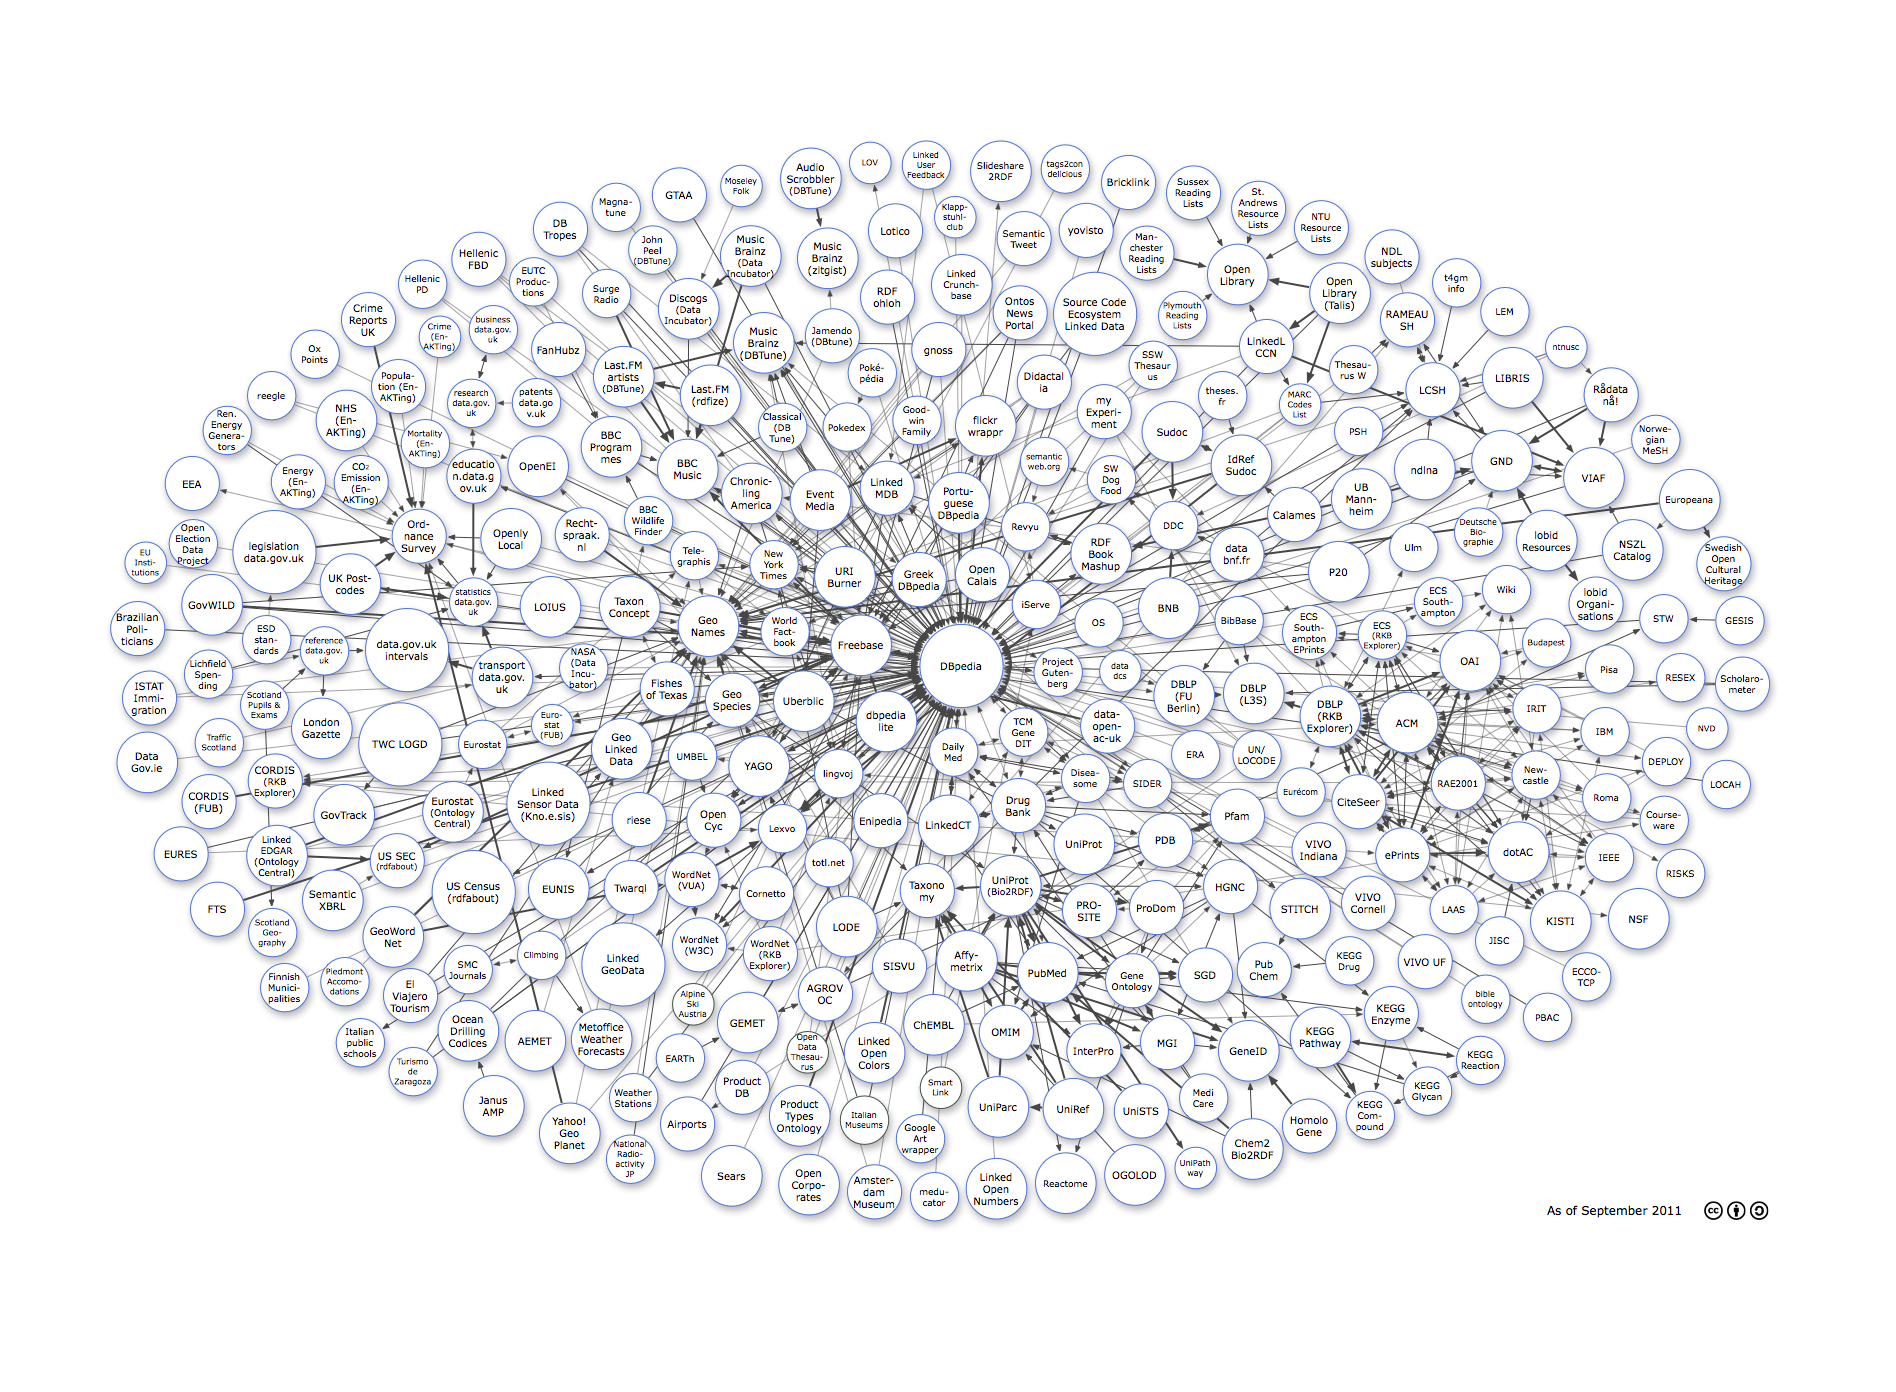
\includegraphics[width=1\linewidth]{./Figures/lod-datasets_2011-09-19.png}
\end{center}
\caption{Linking Open Data cloud diagram, by Richard Cyganiak and Anja Jentzsch. \url{http://lod-cloud.net}}
\label{fig:lod}
\end{figure}

Linked Data is a fundamental part of the Semantic Web essence, facilitating a large scale integration and reasoning
on data on the Web. A typical example of a Linked Data collection is DBpedia
{\footnote{\url{http://www.dbpedia.org/}}}. It basically extracts information from Wikipedia and
makes it available in RDF incorporating links to other datasets on the web, such as 
Geonames\footnote{\url{http://www.geonames.org/}},
YAGO\footnote{\url{http://www.mpi-inf.mpg.de/yago-naga/yago/}}, 
LinkedMDB\footnote{\url{http://www.linkedmdb.org/}} and 
USCensus\footnote{\url{http://www.linkedmdb.org/}}. 
With such linkage, it allows
applications to exploit the extra information these datasets can provide, integrating facts from various different
sources. Figure~\ref{fig:lod} shows the latest version of the whole Linked Open Data cloud
diagram, and Figure~\ref{fig:lodZoom} zooms to and highlights some of the datasets used in this thesis, also sho

\begin{figure}[h!]
\begin{center}
  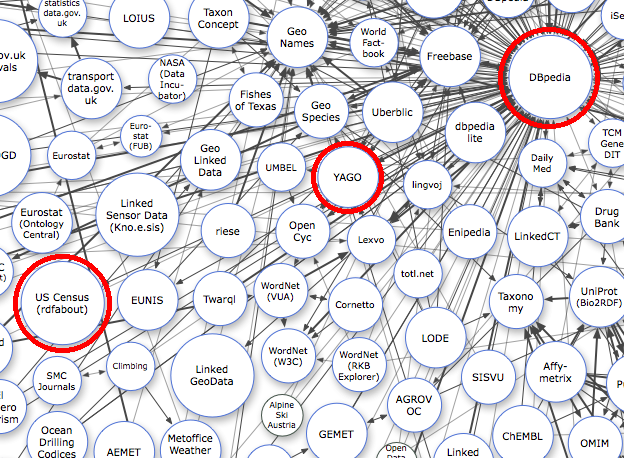
\includegraphics[width=1\linewidth]{./Figures/lod-zoom.png}
\end{center}
\caption{Zoom of Figure~\ref{fig:lod} highlighting datasets relevant to this thesis}
\label{fig:lodZoom}
\end{figure}
 % Related Work

\chapter{\graphname}
\label{ch:intro}

The idea is to build during preprocessing a graph inspired in the Itemset Lattice that describes the influence of different categorical relations on a given numerical attribute's distribution. We call such graph a \graphname.  To illustrate the idea, let's analyze a simple real-world example with the \emph{hasIncome} relation. If we have two categorical relations, one strongly correlated to income, e.g. \emph{hasEducation}, and one uncorrelated (or very weakly correlated), e.g. \emph{wasBornInMonth}.

Let's assume that for the relation \emph{wasBornInMonth(x,y)} we have the 12 months from the Gregorian Calendar as constants and for \emph{hasEducation(x,y)} we can have 10 different categorical constants for \emph{y}: ``Preschool, ``Kindergarten, ``ElementarySchool'', ``MiddleSchool'', ``Highschool'', ``Professional School'', ``Associate's degree'', ``Bachelor's degree'', ``Master's degree'' and ``Doctorate degree''. 

It's expected that the income distribution will be roughly the same for people born in any of the months, whereas for different education levels, e.g. Elementary School and Doctoral Degree, their income distribution are expected to be different between them and different from the overall income distribution.

In a further step, we try to join every possible pair of categorical relations and including the constants. For the given example with the relations \emph{hasEducation} and \emph{wasBornInMonth} we would then create the nodes:

  \emph{hasIncome(x,y)wasBornInMonth(x,``January''),hasEducation(x,``Preschool'')} \newline
  \emph{hasIncome(x,y)wasBornInMonth(x,``January''),hasEducation(x,``Kindergarten'')} \newline
  \dots \newline
  \emph{hasIncome(x,y)wasBornInMonth(x,``January''),hasEducation(x,``Doctorate Degree'')} \newline

  \emph{hasIncome(x,y)wasBornInMonth(x,``February''),hasEducation(x,``Preschool'')} \newline
  \emph{hasIncome(x,y)wasBornInMonth(x,``February''),hasEducation(x,``Kindergarten'')} \newline
  \dots \newline
  \emph{hasIncome(x,y)wasBornInMonth(x,``February''),hasEducation(x,``Doctorate Degree'')} \newline
 
  \dots \newline

  \emph{hasIncome(x,y)wasBornInMonth(x,``December''),hasEducation(x,``Preschool'')} \newline
  \emph{hasIncome(x,y)wasBornInMonth(x,``December''),hasEducation(x,``Kindergarten'')} \newline
  \dots \newline
  \emph{hasIncome(x,y)wasBornInMonth(x,``December''),hasEducation(x,``Doctorate Degree'')} \newline


Based on this idea, we basically check how different categorical relations affect a numerical distribution. Such information, together with other measures like support, provides valuable cues on what categorical attributes and what categorical constants might be the most interesting to be added to the hypothesis in the core ILP algorithm.

\section{Categorical Relation Definition}

In this section, we formally define a categorical relation as used in the \graphname. 

First of all, a candidate relation must be joined with root relation's \ord{1} argument (assuming that the numerical attribute is in the \ord{2} argument). 

A candidate categorical relation $r(x,y)$, should be equivalent a non-injective function:

$r(x,y) \equiv f : X \rightarrow Y ,\, s.t. |Y|<|X| $ and $  |Y|=n ,\, n>1 \newline $
$\nexists \, g : Y \rightarrow X ,\, s.t. f(g(x))=x ,\, \forall x \in X$

We can define subsets of $X_i \in X$, with which of them belonging to one category $y_i \in Y$:

$X_i \subset X ,\, s.t. X_i = \{x \in X \,|\, f(x)=y_i ,\, y_i \in Y\} \newline $
$X = \bigcup_{i=1}^{n} X_i $ and $ X_i \cap X_j = \emptyset ,\, \forall i,j \in [1,n] ,\, i \neq j$

We can also broaden this definition by composing functional relations to a categorical or multiple categorical relations:

If we have:

$r_1(x,y) \equiv f_1 : X \rightarrow Y$ (categorical or not) \newline
$r_2(y,z) \equiv f_2 : Y \rightarrow Z$ (categorical relation)

Then, $r'(x,z) \equiv f : X \rightarrow Z$, where $r'(x,z)=r_2(f_1(x),z)$ is also categorical


Numerical relations can also be turned into a categorical, by simply applying a bucketing function that maps a numerical domain into a finite set of $k$ buckets:

$b: \mathbb{N} \rightarrow B$, where $B=\{b_1,b_2,\dots ,b_k \}$

So a numerical relation:

$r(x,y) \equiv f : X \rightarrow \mathbb{N}$ 

combined with a bucketing function $b$, $r'(x,b(y))$ would be categorical

(Then talk about non-categorical relations as categorical by considering its presence/absence)

\section{Support}

As described in (\cite{LavracDz94}), in top-down ILP every refinement causes the support to decrease, therefore we know that for every node in the \graphname, its support will be greater or equal than any of its children, so support is a monotonically decreasing measure so we can safely prune a node that doesn't reach the minimum support threshold.


\subsection{Independece between Nodes}

By simplicity, we assume that every possible pair of categorical relations are independent and we search for evidence to prove the contrary.

For 2 nodes to be joined, they must have a common parent, i.e. two nodes at level $l$ (with $l+1$ literals) are joinable if they share $l$ literals. Therefore, it's straightforward to calculate the conditional probabilities of each of the joining nodes given the common parent, and estimate the frequency distribution for the conditional independence case.

If we are joining hasEducation()...

Let's say we have the following join case:

\begin{center}
  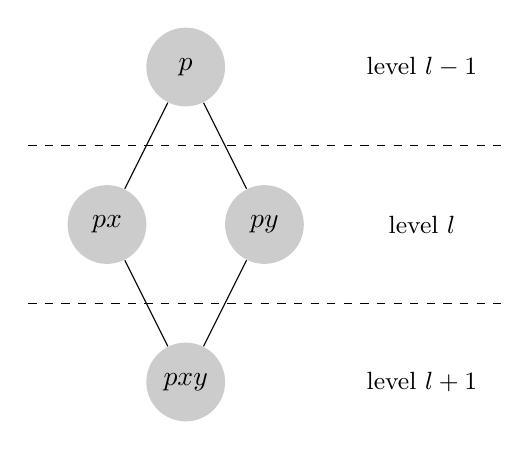
\begin{tikzpicture}
  [scale=1,auto=center,every node/.style={minimum size=1cm}]
    \node (p)  [circle,fill=black!20] at (4,10) {$p$};
    \node (n1) [circle,fill=black!20] at (3,8)  {$p x$};
    \node (n2) [circle,fill=black!20] at (5,8)  {$p y$};
    \node (n12)[circle,fill=black!20] at (4,6)  {$p x y$};


    \foreach \from/\to in {p/n1,p/n2,n1/n12,n2/n12}
      \draw (\from) -- (\to);

    \draw[dashed] (2,9) -- (8,9);
    \draw[dashed] (2,7) -- (8,7);

    \node (level0)[font=\small] at (7,10) {level $l-1$};
    \node (level1)[font=\small] at (7,8)  {level $l$};
    \node (level2)[font=\small] at (7,6)  {level $l+1$};
  \end{tikzpicture}
\end{center}



For every bucket $b_i$, there's a frequency $h_i$ in the histogram, we can calculate the conditional probability $p_i(x|p)$ and $p_i(y|p)$ assuming conditional independence given common parent $p$ in order to estimate $\hat{h_i}(p x y)$:

\begin{equation}
\begin{split}
 p_i(x|py) &= p_i(x|p) \\ 
 &= \cfrac{h_i(x)}{h_i(p)} \\ 
 p_i(y|px) &= p_i(y|p) \\ 
 &= \cfrac{h_i(y)}{h_i(p)} \\ \\ 
 \hat{h_i}(pxy) &= p_i(x|py)p_i(y|p)*h_i(p) \\ 
 &= p_i(x|p)h_i(y) \\ 
 \hat{h_i}(pxy) &= p_i(y|px)p_i(x|p)*h_i(p) \\ 
 &= p_i(y|p)h_i(x) 
\end{split}
\end{equation}

After that, we query the actual frequency distribution on the Knowledge Base and do an Pearson's chi-squared independence test. As null hypothesis and alternative hypothesis we have:

\begin{itemize}
 \item $H_0$ = \emph{$x$ and $y$ are conditionally independent given their common parent $p$}
 \item $H_1$ = \emph{$x$ and $y$ are conditionally dependent given their common parent $p$} 
\end{itemize}

  

Number of degrees of freedom is the number of buckets minus one:

\begin{center}
 $df=k-1$
\end{center}

We calculate the $\chi^2$ value:

\begin{equation}
 \chi^2=\sum_{i=1}^{k} \cfrac{(h_i - \hat{h_i})^2}{\hat{h_i}}
\end{equation}

\cite{Jaroszewicz02pruningredundant}

Then it's possible to obtain the p-value and check whether there's enough confidence to reject the null hypothesis $H_0$. In level 1 from \graphname, nodes can be directly pruned, on the other hand, for further levels, for a node to be pruned by independence, all the possible joins resulting the node must be independent. In level 2, for example, in order to prune the node $r a_1 b_1 c_1$, given that in level 1 the nodes $r a1 b1$, $r a1 c1$ and $r b1 c1$ were not pruned. All the three possible join combinations should fail the independence test, i.e.:

\begin{equation}
\begin{split} 
  freq(r a_1 b_1 c_1) &\approx freq(r a_1)p (r b_1|r a_1) p(r c_1|r a_1) \\ 
  &\approx  freq(r b_1) p(r a_1|r b_1) p(r c_1|r b_1) \\ 
  &\approx  freq(r c_1) p(r a_1|r c_1) p(r b_1|r c_1)  
\end{split}
\end{equation}

This applies to nodes at any level $l$, with $p \leq l$ parents and $C_{2}^{p}$ possible join pairs.

\section{Heuristics}

As seen in the previous sections, the number of nodes in \graphname grow exponentially with the number of categorical relations and its constants. For $n$ categorical relations, each with $m$ constants, the total number of nodes is $2^{n*m}$. Frequently, pruning by support and independence is not sufficient to make it feasible and it's necessary to apply heuristics to prune more aggressively.

As we are interested in categories that produces a subsets with a distribution different from the root and its super-categories (parent nodes, for the case of joining multiple categories), distribution divergence measures are a good option. Some of the state-of-the-art measures we can use are the following:

\begin{itemize}
 \item Kullback-Leibler \cite{Kullback51klDivergence}: 
    \begin{equation}
      D_{KL}(P||Q)=\sum_{\substack{i}}\ln\left(\cfrac{P(i)}{Q(i)}\right)*P(i)
    \end{equation}
 \item Chi-squared ($\chi^2$):
    \begin{equation}
      D_{\chi^2}(P||Q)=\sum_{\substack{i}}\cfrac{(P(i)-Q(i))^2}{P(i)}
    \end{equation}
 \item Jensen-Shannon \cite{17795}:
    \begin{equation}
      D_{JS}(P||Q)=\cfrac{1}{2}D_{KL}(P||M)+\cfrac{1}{2}D_{KL}(Q||M), 
    \end{equation}
\end{itemize}

Where $P$ and $Q$ are the distributions to be compared and $M=\cfrac{1}{2}(P+Q)$

As discussed in \cite{17795}, although Jensen-Shannon is computationally more expensivee, it has the advantage of being a symmetric and smoothed version of the Kullback-Leibler measure.

Nevertheless, using a divergence measure alone might also be problematic. Nodes with low support are very likely to present high divergence and when 






\chapter{Algorithmic Framework}
\label{ch:intro}

\section{Knowledge Base Backend}

\cite{Neumann:2010:RES:1731351.1731354}

\section{Preprocessing}

In this section, we will present the preprocessing steps required by our proposed algorithm. It basically consists of building a joinable relations map for each of the four join patterns, according to relations domain and range types as well as support threshold. Afterwards, we search the available categorical properties for each numerical relation that will be used in the \graphname. At last we describe the \graphname structure and the algorithm to build it.

\subsection{Relation Preprocessing}

In this step, we focus on creating for each of the four join patterns between two relations:

\begin{itemize}
 \item Argument 1 on Argument 1: e.g. \emph{hasIncome(\textbf{x},y)hasAge(\textbf{x},z)}
 \item Argument 1 on Argument 2: e.g. \emph{hasIncome(\textbf{x},y)isMarriedTo(z,\textbf{x})}
 \item Argument 2 on Argument 1: e.g. \emph{livesIn(y,\textbf{x})isLocatedIn(\textbf{x},z)}
 \item Argument 2 on Argument 2: e.g. \emph{livesIn(y,\textbf{x})wasBornIn(z,\textbf{x})}
\end{itemize}



\subsubsection{Exploiting Relation Range and Domain Types}

A knowledge base is expected to have an ontology defining the structure of the stored data (the types of entities and their relationships). Additionally, every relation's range (type of \ord{1} argument) and domain (type of \ord{2} argument) should be defined. These information can help us identify the allowed joining relations for each join pattern.

For every possible pair of relations, 

The algorithm is shown in the pseudo-code bellow:

\begin{algorithm}[5]
 \caption{Checks whether two relations are joinable for a given join pattern}
 \SetKwFunction{subsumes}
 \KwIn{Relation $r_i$, $r_j$, Argument $arg_i$, $arg_j$}
 \KwOut{True if $arg_i$ from $r_i$ joins with $arg_j$ from $r_j$, False otherwise}
 
  \eIf{$r_i.arg_i = r_j.arg_j$ {\bf or} \FuncSty{subsumes(}$r_i.arg_i$,$r_j.arg_j$\FuncSty{)} {\bf or} \FuncSty{subsumes(}$r_j.arg_j$,$r_i.arg_i$\FuncSty{)}}{
      \Return true\;
   }{
    \Return false\;
  }
\end{algorithm}

\subsubsection{Exploiting Support Monotonicity}

As seen in (???), support is the only monotonically decreasing measure in top-down ILP. So we know that by adding any literals to the hypothesis, we can only get a smaller or equal support. Therefore, for each pair of joinable relations in each of the join patterns, we can query the knowledge base and check whether they reach the minimum support threshold.

Thus, if any pair of relations doesn't reach the minimum support for a given join pattern, we know that any hypothesis containing such join will therefore fail the support test as well, so we don't need to test such hypothesis in the core ILP algorithm.


\begin{algorithm}
  \caption{Checks valid join pairs for a given join patterns}
  %\begin{algorithmic}
 % \Function {checkJoinSupport}{r_i,r_j,arg_i,arg_j,supportThreshold}
 %     \If{r_i.arg_i = r_j.arg_j \or subsumes(r_i.arg_i,r_j.arg_j) \or subsumes(r_j.arg_j,r_i.arg_i)}
%	  \Return true 
 %     \Else
%	  \Return false
 %     \EndIf
  %\EndFunction
  
  %\end{algorithmic}
\end{algorithm}


The relation preprocessing will result in 4 maps, one for each join pattern. Each map will a relation as key and a set of joinable relations as value. The refinement step at the ILP algorithm, will then access this map when choosing a new literal to be added.


\subsection{\graphname}

\subsubsection{Graph Node}

Every node essentially contains the following attributes:

\begin{itemize}
 \item Set of pointers to parent nodes
 \item Set of pointers to child nodes
 \item Set of pointers to constant nodes
 \item Histogram with facts distribution over root numerical property
\end{itemize}


\subsubsection{Building the \graphname}

For building the \graphname, we start with the root node, which has a numerical property as literal and no constants assigned, e.g. \emph{hasIncome(x,y)}. We then query the  distribution of positive examples over the property in the whole Knowledge Base.

\begin{center}
 \emph{SELECT COUNT ?y WHERE \{ ?x <hasIncome> ?y \} GROUP BY (?y)}
\end{center}

It's also necessary to specify the bucketing technique and the number of buckets in order to extract the histogram from the obtained query results. These buckets are used to build the histograms of all nodes in the graph.

Afterwards, we select the the categorical properties that will be used in the lattice. For each of the selected properties, we join them with the root numerical property (for simplicity we'll assume all the categorical properties are joined with both \ord{1} arguments) and we query the distribution again. In the first level, it's necessary to extract a histogram for each of the categorical constants in the selected properties. Therefore, it's a good strategy to group the results also by these categorical constants so If we select \emph{hasEducation} for example, we would then fire the following SPARQL query:

\begin{center}
 \emph{SELECT COUNT ?z ?y WHERE \{ ?x <hasIncome> ?y . ?x <hasEducation> ?z \} GROUP BY (?z,?y)}
\end{center}

With such query, it's possible to extract a histogram for the node \emph{hasIncome(x,y)hasEducation(x,z)} and its correspondent constants 

\subsubsection{Searching Rules in \graphname}

\subsubsection{}



\section{ILP Core Algorithm}


 % Data Model

%\input{./Chapters/Chapter4} % CATE Framework

%\input{./Chapters/Chapter5} % Information Extraction

%\input{./Chapters/Chapter6} % Context-Aware Ranking

%\input{./Chapters/Chapter7} % Implementation

%\input{./Chapters/Chapter8} % Experiment

%\input{./Chapters/Chapter9} % Conclusion

%% ----------------------------------------------------------------
% Now begin the Appendices, including them as separate files

\addtocontents{toc}{\vspace{2em}} % Add a gap in the Contents, for aesthetics

%% ----------------------------------------------------------------
%\lhead{\emph{List of Figures}}  % Set the left side page header to "List if Figures"
\listoffigures  % Write out the List of Figures

%% ----------------------------------------------------------------
%\lhead{\emph{List of Tables}}  % Set the left side page header to "List of Tables"
\listoftables  % Write out the List of Tables

\appendix % Cue to tell LaTeX that the following 'chapters' are Appendices

%% Appendix A

\chapter{Appendix Title Here}
\label{AppendixA}
%\lhead{Appendix A. \emph{Appendix Title Here}}

Write your Appendix content here.	% Appendix Title

%\input{./Appendices/AppendixB} % Appendix Title

%\input{./Appendices/AppendixC} % Appendix Title

\addtocontents{toc}{\vspace{2em}}  % Add a gap in the Contents, for aesthetics
\backmatter

%% ----------------------------------------------------------------
\label{Bibliography}
%\lhead{\emph{Bibliography}}  % Change the left side page header to "Bibliography"
\bibliographystyle{unsrtnat}  % Use the "unsrtnat" BibTeX style for formatting the Bibliography
\bibliography{Bibliography}  % The references (bibliography) information are stored in the file named "Bibliography.bib"

\end{document}  % The End
%% ----------------------------------------------------------------